%%%%%%%%%%%%%%%%%%%%%%%%%%%%%%%%%%%%%%%%%%%%%%%%%%%%%%%%%%%%%%%%%%%%%%%%%%
%% Trim Size: 10.25in x 7.5in            %Raj - 09 Feb 2004
%% Text Area: 8.5in (include Runningheads) x 6in
%% ws-jca.tex   :  23-5-2008
%% Tex file to use with ws-jca.cls written in Latex2E.
%% The content, structure, format and layout of this style file is the
%% property of World Scientific Publishing Co. Pte. Ltd.
%% Copyright 1995, 2003 by World Scientific Publishing Co.
%% All rights are reserved.
%%%%%%%%%%%%%%%%%%%%%%%%%%%%%%%%%%%%%%%%%%%%%%%%%%%%%%%%%%%%%%%%%%%%%%%%%%%%

\documentclass{ws-jca}
\usepackage{graphicx} 
\usepackage{color}

\newcommand{\threeD}{3\nobreakdash\textendash D }	% for "3-D'' with no break
\newcommand{\twoD}{2\nobreakdash\textendash D }	% for "2-D'' with no break
\newcommand{\twoDxN}{2\nobreakdash\textendash DxN }
\newcommand{\Cerveny}{\v{C}erven\'{y} }

\renewcommand{\thefootnote}{\fnsymbol{footnote}}

\begin{document}

\markboth{S. M. Reilly, G. Potty}
{Verification Tests for Hybrid Gaussian Beams in Spherical/Time Coordinates}

%%%%%%%%%%%%%%%%%%%%% Publisher's Area please ignore %%%%%%%%%%%%%%%
%
\catchline{}{}{}{}{}
%
%%%%%%%%%%%%%%%%%%%%%%%%%%%%%%%%%%%%%%%%%%%%%%%%%%%%%%%%%%%%%%%%%%%%

\title{Verification Tests for Hybrid Gaussian Beams in Spherical/Time Coordinates}

\author{Sean M. Reilly}
\address{Department of Ocean Engineering, University of Rhode Island,\\
Narragansett RI, USA\\
\email{campreilly@my.uri.edu} }

\author{Gopu Potty}
\address{Department of Ocean Engineering, University of Rhode Island,\\
Narragansett RI, USA\\
\email{potty@egr.uri.edu} }

\maketitle

\begin{history}
\received{(Day Month Year)}
\revised{(10 May 2012)}
\end{history}

\begin{abstract}
The previous paper defined a new undersea acoustic propagation loss model
that is specifically designed to support real-time, sonar
simulation/stimulation systems, in littoral environments, at active sonar
frequencies. This paper seeks to verify the model's implementation by
comparing the modeled results to analytic solutions.
\end{abstract}

\keywords{Gaussian beams, 3--D modeling, range-dependent, time-domain.}

\section{Introduction}

The previous paper\cite{Reilly2012} defined the theory for a new undersea
acoustic propagation loss model that is specifically designed to support
real-time, sonar simulation/stimulation systems, in littoral environments,
at active sonar frequencies. The WaveQ3D model implements this theory using
a circular queue of time domain wavefronts, in a fully 3-D ocean
environment, with a computationally-efficient form of C++ vector
processing.\cite{Veldhuizen1995} This follow-up paper analyzes the
capabilities and limitations of this implementation. The Capability
Maturity Model Integration (CMMI)\cite{Chrissis2007} separates testing
needed for such an effort into two phases:
\begin{itemize}
\item {\bf Verification} testing ensures that selected work products meet
their specified requirements. For this analysis, the WaveQ3D model is
decomposed into its component parts (such as ray tracing, reflection,
eigenray finding, and propagation loss), and the results from each parts
are compared to analytic solutions.
\item {\bf Validation} testing demonstrates that a product or product
component fulfills its intended use when placed in its intended
environment. For the WaveQ3D model, this will consist of comparisons to
real-world results in a subsequent paper.
\end{itemize}
Decomposing the testing in this way is designed to ensure that any
conclusions drawn from the modeled results rest on a firm foundation of
understanding.

\section{Ray Tracing Tests}

The ray paths in this model use a third order Adams-Bashforth (AB3)
marching solution\cite{Yakowitz1986} to create a circular queue of time
domain wavefronts. The evolution of the wavefront shape, as it passed
through the 3-D ocean environment, is defined by the following equations.
\begin{equation}
	\frac{dr}{dt} = c^2 \alpha \:,
	\label{eq:dr_dt}
\end{equation}
\begin{equation}
	\frac{d\theta}{dt} = \frac{c^2 \beta}{r} \:,
	\label{eq:dtheta_dt}
\end{equation}
\begin{equation}
	\frac{d\phi}{dt} = \frac{c^2\gamma}{r \sin{\theta}} \:,
	\label{eq:dphi_dt}
\end{equation}
\begin{equation}
	\frac{d\alpha}{dt} = -\frac{1}{c}\frac{dc}{dr} 
		+ \frac{c^2}{r}\left( \beta^2 + \gamma^2 \right) \:,
	\label{eq:dalpha_dt}
\end{equation}
\begin{equation}
	\frac{d\beta}{dt} = -\frac{1}{c \: r}\frac{dc}{d\theta} 
		- \frac{c^2}{r} \left( \alpha \beta + \gamma^2 cot\theta \right) \:.
	\label{eq:dbeta_dt}
\end{equation}
\begin{equation}
	\frac{d\gamma}{dt} = -\frac{1}{c \: r \sin{\theta}}\frac{dc}{d\phi} 
		- \frac{c^2 \gamma}{r} \left( \alpha + \beta \cot{\theta} \right) \:,
	\label{eq:dgamma_dt}
\end{equation}
where 
$c$ is the speed of sound as a function of location;
$t$ is the travel time;
\((r, \theta, \phi)\) are the spherical earth coordinates of the modeled ray 
path as a function of time; and
\((\alpha, \beta, \gamma)\) are the spherical earth coordinates of the 
normalized ray direction as a function of time.
The tests discussed in this section analyze the accuracy of
Eqs.~(\ref{eq:dr_dt}) through (\ref{eq:dgamma_dt}) in scenarios where the
rays do not encounter any boundaries.

\subsection{Comparisons to ``flat earth'' benchmarks}

Because WaveQ3D is one of the few models to use non-Cartesian coordinate
system, comparisons to other work often require translation before
differences can be analyzed. This section analyzes the accuracy of the
translation between spherical and Cartesian coordinate models. Cartesian
coordinate propagation models frequently use a modified index of
refraction\cite{Pekeris1946} to incorporate earth curvature effects into
their calculations.
\begin{equation}
	n'(r) = \frac{r}{R} \frac{n(r)}{n(R)} \:, 
\end{equation}
\begin{equation}
	c'(z) = \frac{c(z)}{1-z/R} \:, 
\end{equation}
where
$R$ is the radius of earth's curvature in this area of operations;
$r$ is the radial distance from the center of curvature (positive is up);
$z = R-r$ is the below the ocean surface (positive is down);
$n(z), n'(z)$ are the original and modified index of refraction, and
$c(z), c'(z)$ are the original and modified speed of sound.
When a testing benchmark is specified in Cartesian coordinate, the inverse of this
process must be implemented to create an equivalent environment in
spherical earth coordinates.
\begin{equation}
	c'(r) = \frac{r}{R} \: c(r) \:, 
	\label{eq:cflat_adjustment}
\end{equation}
where $c(r)$ is the benchmark's original $c(z)$ sound speed converted to a
function of $r$.

The Munk profile\cite{Munk1974} was used to evaluate the accuracy of
testing Cartesian benchmarks in a model based on spherical earth
coordinates. The Munk profile is an idealized representation of a typical
deep sound channel, and it was chosen for its ability to support long range
paths without interface reflection. 
\begin{equation}
	z' = 2 \frac{z-z_1}{B} \:,
	\label{eq:munk_zprime}
\end{equation}
\begin{equation}
	c(z) = c_1 \left[ 1 + \epsilon \left( z' - 1 + e^{-z'} \right) \right] \:,
	\label{eq:munk_profile}
\end{equation}
where
$z'$ is the normalized depth (positive is down),
\(z_1\) is the depth of the deep sound channel axis (1300 meters),
$B$ is a depth scaling factor (1300 meters),
\(c_1\) is the sound speed on deep sound channel axis (1500~m/s), and
\(\epsilon\) is the profile scaling factor (7.37x10\textsuperscript{-3}).
The specific Munk profile parameters used in this test were selected to
match Fig.~3.19 in Jensen, Kuperman, et. al.\cite{Jensen1994,Porter1997} An
example of the ray paths for this profile are illustrated in
Fig.~\ref{fig:munk_rays}. This figure was created by WaveQ3D with a 100~ms
time increment and 1\textsuperscript{o} separated depression/elevation
launch angles from -14\textsuperscript{o} to 14\textsuperscript{o}. Launch
angles greater than 14.38\textsuperscript{o} encounter interface
reflections.
\begin{figure}[th]
	\centerline{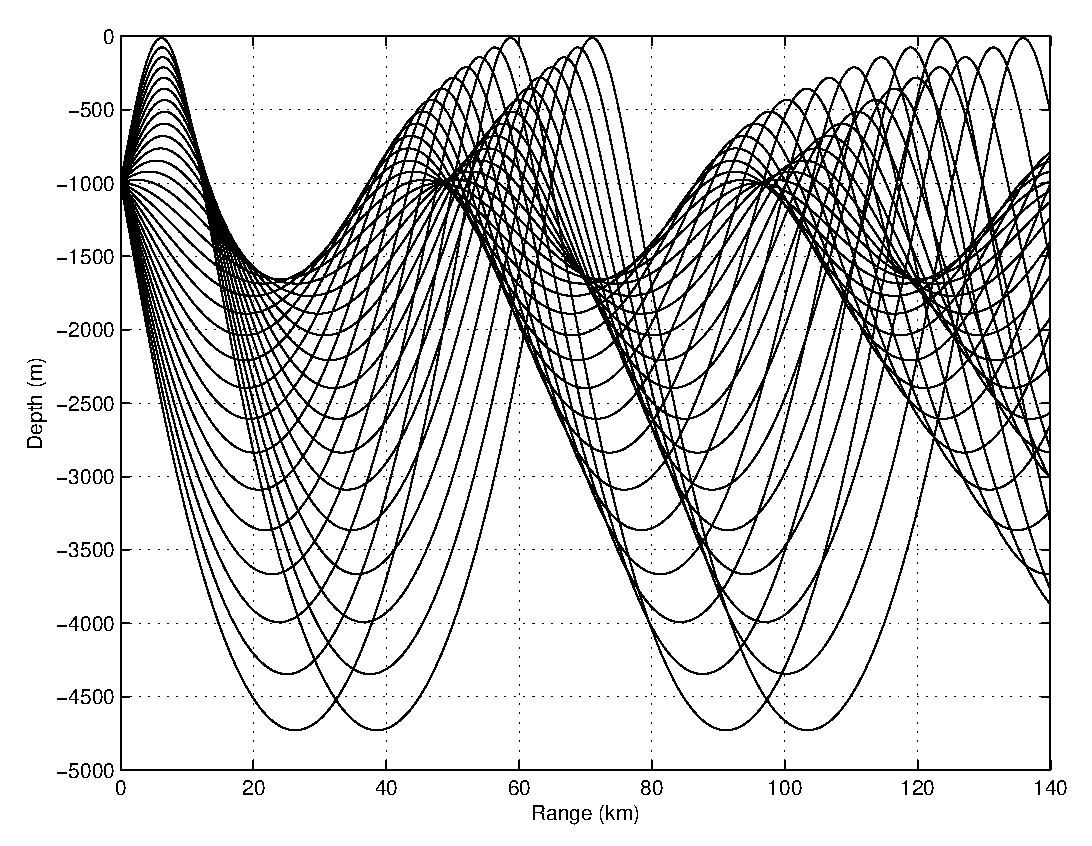
\includegraphics[width=3in]{refraction_munk_range_wave.eps}} 
	\vspace*{8pt}
	\caption{Modeled ray paths for the Munk profile. 
	\label{fig:munk_rays}}
\end{figure}

Munk's paper\cite{Munk1974} characterized the analytic solution for ray
paths using their cycle range, the range required to complete one period of
upward and downward refraction. The cycle range is equal for positive and
negative launch angles. The cycle range was used as the metric for this test
because it could be cast into identical units in both spherical and Cartesian
coordinates. 

To create an analytic equivalent to a typical Cartesian model, Snell's Law
(Eq. \label{eq:snells_cart}) was integrated numerically, using the
MATLAB\texttrademark quadgk() implementation of an adaptive Gauss-Kronrod
quadrature.\cite{Shampine2010}
\begin{equation}
	a = \frac{\cos{\eta(z)}}{c(z)} = \text{constant} \:,
	\label{eq:snells_cart}
\end{equation}
\begin{equation}
	\frac{dH}{dz} =  \frac{\cos{\eta(z)}}{\sin{\eta(z)}} \:,
	\label{eq:snells_cart_slope}
\end{equation}
\begin{equation}
	\Delta H = \int_{z_s}^{z_t} \frac{ a c(z) }{ \sqrt{ 1-(a c(z))^2 } } \: dz \:,
	\label{eq:snells_cart_integ}
\end{equation}
\begin{equation}
	\Delta t = \int_{z_s}^{z_t} \frac{1}{ c(z) \sqrt{ 1-(a c(z))^2 } } \: dz \:,
	\label{eq:snells_cart_time_integ}
\end{equation}
where
\(\eta(z)\) is the depression/elevation angle along the ray path;
$a$ is the ray parameter (constant for each launch angle);
\(H\) is the horizontal range;
\(t\) is the travel time;
\(z_s\) is the source depth; and
\(z_t\) is the target depth.
Although these integrals only apply between the source and the first vertex
or reflection, paths out to any range can be constructed by repeating this
process after the vertex or reflection.

To create equivalent conditions for a model based on spherical earth
coordinates, we modified the original sound speed using
Eq.~(\ref{eq:cflat_adjustment}), and then performed a similar integration
in spherical coordinates. Snell's law in spherical media includes an extra
factor of $r$ that is not present in the Cartesian
coordinates.\cite{Cerveny2001} The slope of the ray path also includes an
extra factor of$r$ in spherical coordinates.
\begin{equation}
	p = \frac{r \cos{\eta(r)}}{c(r)} = constant
	\label{eq:snells_sphr}
\end{equation}
\begin{equation}
	\frac{r d\theta}{dr} = \frac{\cos{\eta(r)}}{\sin{\eta(r)}}
	\label{eq:snells_sphr_slope}
\end{equation}
\begin{equation}
	\Delta \theta = \int_{r_s}^{r_t} \frac{ p c(r) }{ r \sqrt{ r^2-(p c(r))^2 } } dr
	\label{eq:snells_sphr_integ}
\end{equation}
\begin{equation}
	\Delta t = \int_{r_s}^{r_t} \frac{ r }{ c(r) \sqrt{ r^2-(p c(r))^2 } } dr
	\label{eq:snells_sphr_time_integ}
\end{equation}
where
\(\eta(r)\) is the depression/elevation angle along the ray path;
$p$ is the ray parameter for spherical media (constant for each launch angle),
\(\Delta \theta \) is the horizontal range in solid angle units;
\(r_s\) is the radial coordinate for the source depth; and
\(r_t\) is the radial coordinate for the target depth.

The difference in the cycle ranges computed using these two analytic
solutions is shown in \ref{fig:flattening_accuracy}. The results were
computed for two complete periods, with launch angles from
0\textsuperscript{o} to 14\textsuperscript{o}, as a function of the
spherical coordinates cycle range solution. The 0\textsuperscript{o} launch
angle has difference of -5.14 meters at a range of 96.16 km. The
14\textsuperscript{o} launch angle has a has difference of -38.34 meters at
range of 129.95 km. The intermediate angles have monotonically increasing
values between those two extremes.
\begin{figure}[th]
	\centerline{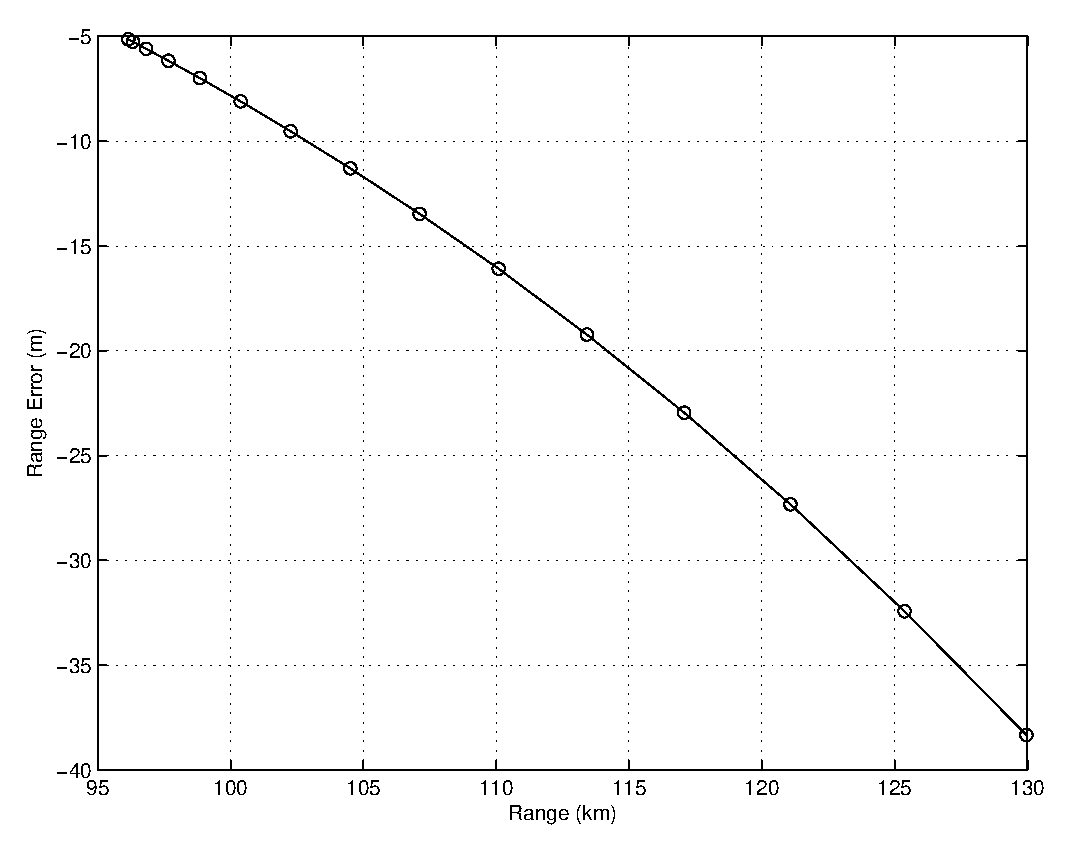
\includegraphics[width=3in]{munk_range_compute.eps}} 
	\vspace*{8pt}
	\caption{earth-flattening accuracy for the Munk profile. 
	\label{fig:flattening_accuracy}}
\end{figure}

Since both solutions are analytic, we conclude that difference must be a
fundamental property of ray paths computations in the two coordinate
systems. It is equally valid to attribute these results to
\begin{itemlist}
\item Errors created by a spherical model working with a Cartesian environment, or
\item Errors created by a Cartesian model working with a spherical environment.
\end{itemlist}
The second case is more interesting for this study, because it represents a
widely accepted (but seldom mentioned) lower limit on ray path range
accuracy, approximately 0.03\% of the total range.

\subsection{Ray path accuracy in a deep sound channel}

In this test, the refraction accuracy of the WaveQ3D model was computed for
a ``flat earth'' Munk profile defined in spherical coordinates by combining
Eqs.~(\ref{eq:munk_zprime}) and (\ref{eq:munk_profile}) with
Eq.~(\ref{eq:cflat_adjustment}). Fig.~\ref{fig:refraction_munk_range}
illustrates the difference between individual WaveQ3D rays and the
spherical analytic solution defined by Eqs.~(\ref{eq:snells_sphr}) through
(\ref{eq:snells_sphr_integ}). Cycle ranges were computed for both the first
and second period of the SOFAR cycle. Because both solutions were computed
in spherical coordinates, using the same sounds speed profile, these error
can not be attributed to the use of a modified index of refraction.
\begin{figure}[th]
	\centerline{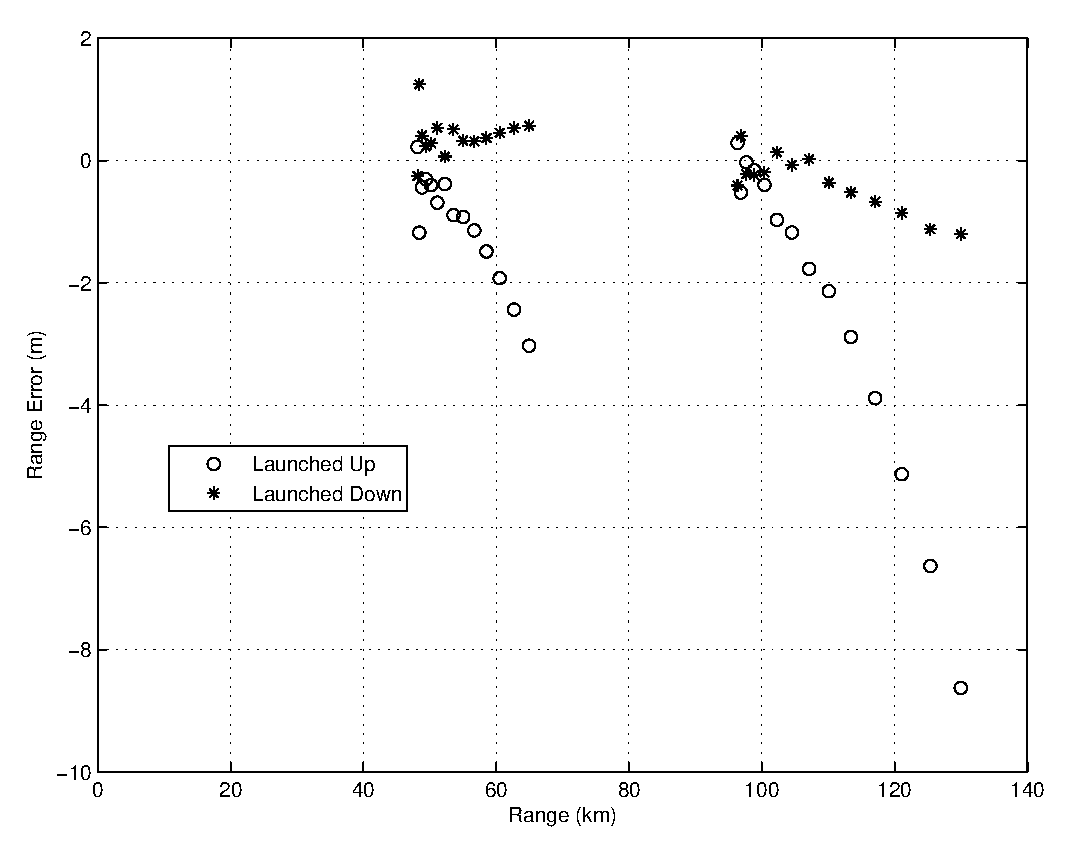
\includegraphics[width=3in]{refraction_munk_range.eps}} 
	\vspace*{8pt}
	\caption{WaveQ3D errors for the Munk profile. 
	\label{fig:refraction_munk_range}}
\end{figure}

With a 100 ms step size, the WaveQ3D result deviates from the analytic
solution by a maximum of -8.62 meters at cycle range of 129.95 km (0.007\%
error). However, 50 out of 58 samples (86\%) exhibited errors less than
\(\pm\) 2 meters (0.002\% error). Ray paths that were initially launched
toward the surface, where the sound speed gradient is highest, had
consistently larger errors than paths that were launched down. The fact
that these errors were all significantly less than those of associated with
the earth curvature correction (Fig.~\ref{fig:flattening_accuracy})
suggests that WaveQ3D model's cycle range estimate meets or exceeds the
accuracy of Cartesian models used on a spherical earth.
\begin{figure}[th]
	\centerline{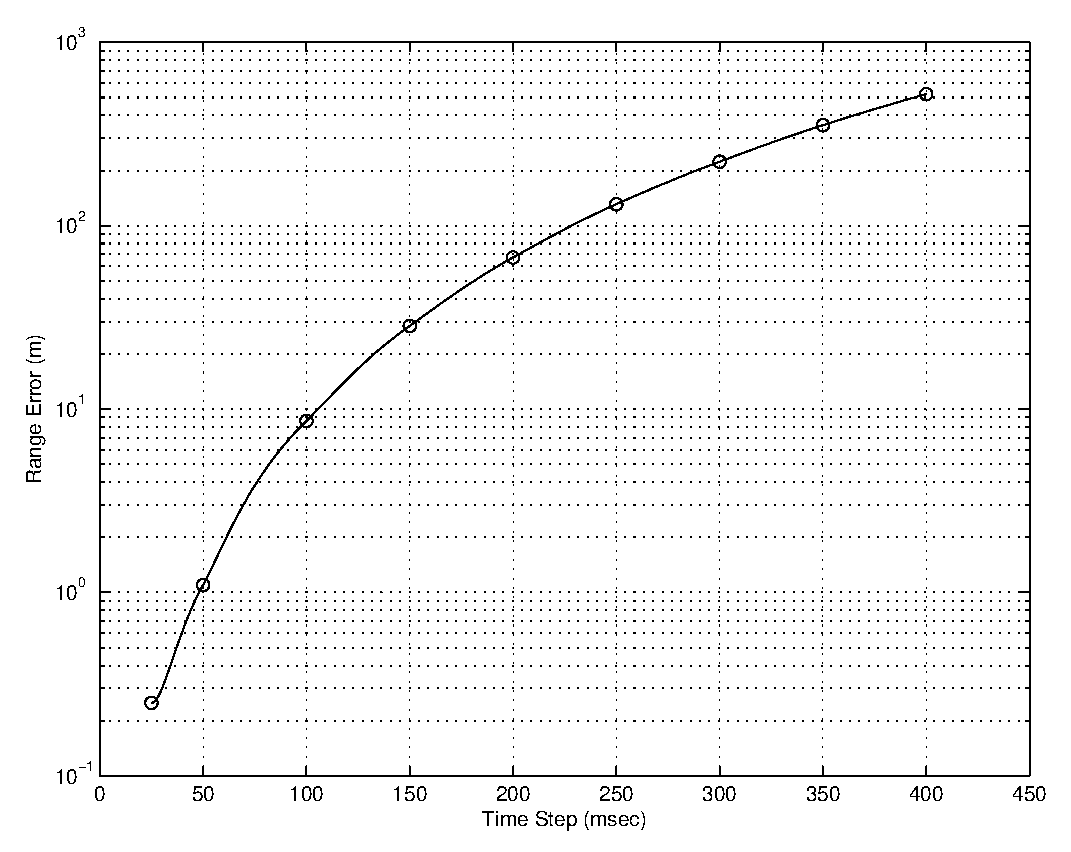
\includegraphics[width=3in]{refraction_munk_sensitivity.eps}} 
	\vspace*{8pt}
	\caption{Path accuracy sensitivity to step size for the Munk profile. 
	\label{fig:refraction_munk_sensitivity}}
\end{figure}

To estimate the impact of WaveQ3D options on this result, the maximum error
was also computed as a function of time step size. The circles in
Fig.~\ref{fig:refraction_munk_sensitivity} represent maximum errors, across
launch angles, for time steps of 25, 50, 100, 150, 200, 250, 300, 350, and
400~ms. The connecting lines smoothly interpolate between these discreet
values. From this, we conclude that the accuracy of WaveQ3D cycle range
estimates is slightly weaker than a power law; a doubling of the time step
decreased the accuracy by approximately a factor of 10. Step sizes as large
as 150 yielded results that were at least as accurate as errors associated
with the modified index of refraction. Given that some environments may
have stronger gradients than the Munk profile, we conclude that a 100 ms
step size should be adequate for most long range applications.

\subsection{Ray path accuracy in an extreme downward refraction environment}

In this test, the refraction accuracy of the WaveQ3D model was computed for the
extreme n\textsuperscript{2}~linear test case developed by Pedersen and
Gordon.\cite{Pedersen1972}
\begin{equation}
	c(z) = \frac{c_0}{\sqrt{1+\frac{2 g_0}{c_0}z}}
	\label{eq:pedersen_profile}
\end{equation}
where
\(c_0\) is the sound speed at the ocean surface (1550 m/s); 
\(g_0\) is the sound speed gradient at at the ocean surface (1.2 s\textsuperscript{-1}).
At shallow depths, this profile matches observed conditions from the
Pacific, in an area of extreme velocity gradient. But at depths greater
than about 60 meters, it predicts theoretically useful, but physically
unrealistic sound speeds. This profile was selected for this study because
of its wide use by other authors in the testing of Gaussian beam model
behavior at the edge of a shadow zone.\cite{Porter1987,Weinberg1996} (Note
that the specific values for this profile parameters were selected to match
the MKS representation of Eq.~3.47 in Jensen, Kuperman, et.
al.\cite{Jensen1994} instead of the English units used in the original
Pedersen and Gordon paper.) 

\begin{figure}[th]
	\centerline{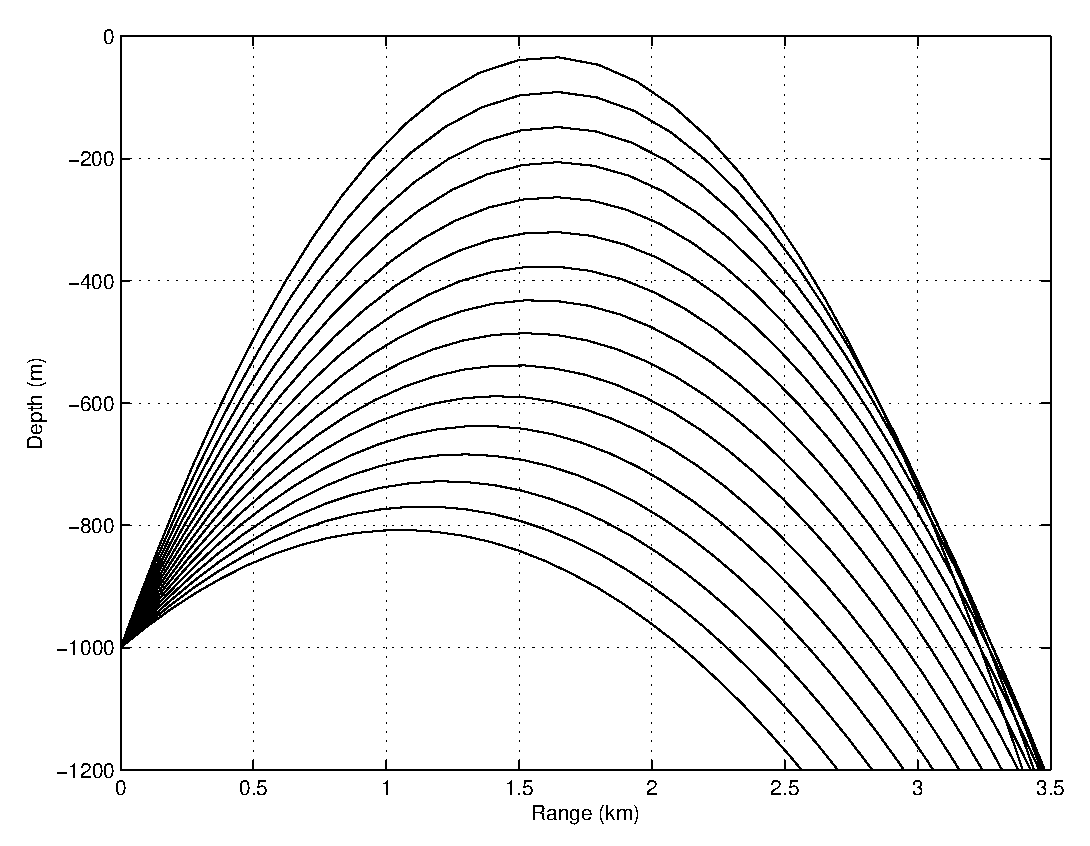
\includegraphics[width=3in]{refraction_pedersen_range_wave.eps}} 
	\vspace*{8pt}
	\caption{Modeled ray paths for the Pedersen/Gordon profile. 
	\label{fig:refraction_pedersen_range_wave}}
\end{figure}
The ray paths to be tested for this profile are illustrated in
Fig.~\ref{fig:refraction_pedersen_range_wave}. This figure was created by
WaveQ3D with a 100~ms time increment and 1\textsuperscript{o} separated
depression/elevation launch angles from 20\textsuperscript{o} to
50\textsuperscript{o}. A ``flat earth'' adjustment was applied to Eqn.
\ref{eq:pedersen_profile} to allow these results to be similar to those
computed in Cartesian coordinates. Launch angles greater than
51.21\textsuperscript{o} encounter interface reflections. The rays launched
at angles between 44\textsuperscript{o} and 50\textsuperscript{o} travel
through a caustic and cross the direct path rays. Because the ray paths
were not periodic, we redefined the cycle range as the horizontal
range needed to travel up to the first vertex and back to the source depth.
Figure~\ref{fig:refraction_pedersen_range} illustrates the difference
between individual WaveQ3D rays and the spherical analytic solution defined
by Eqs.~(\ref{eq:snells_sphr}) through (\ref{eq:snells_sphr_integ}). The
WaveQ3D model had a maximum error of 1.3~m at cycle range of 2595.1~m
(0.05\% error), but there appeared to be a slight bias. We discovered that
many of the launch angles had cycle range errors right around -0.5~m.
\begin{figure}[th]
	\centerline{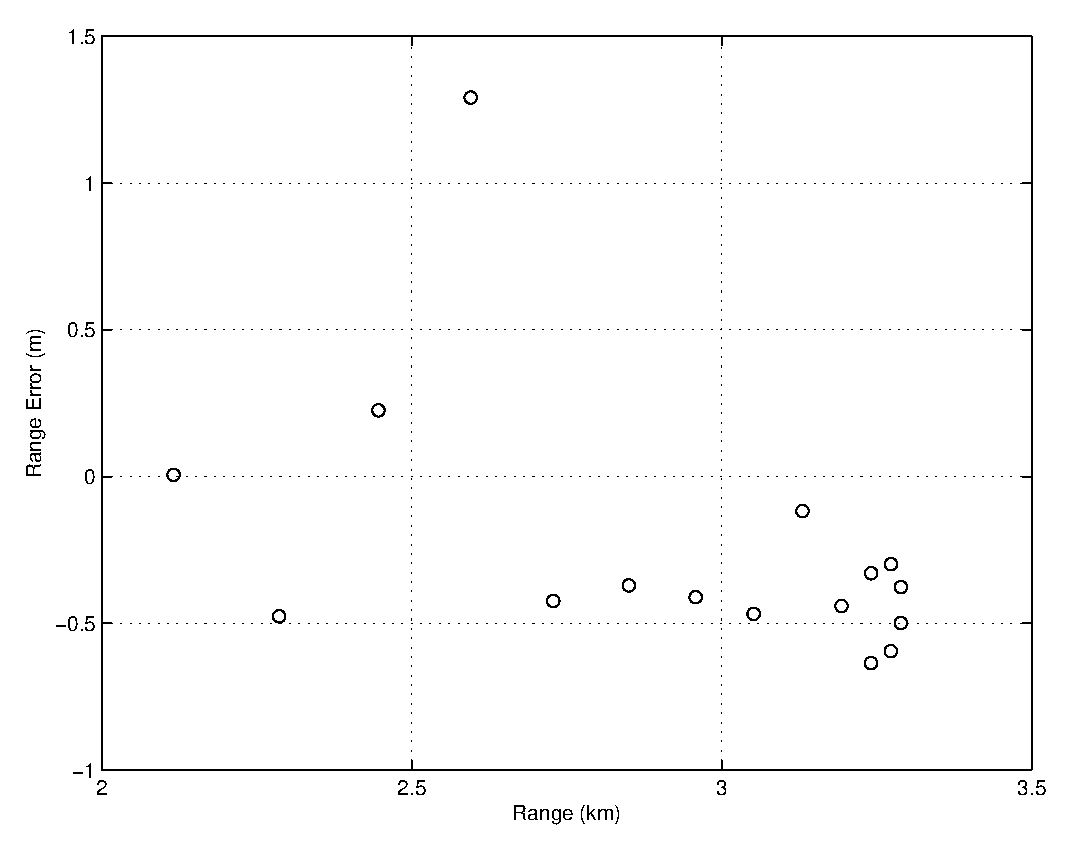
\includegraphics[width=3in]{refraction_pedersen_range.eps}} 
	\vspace*{8pt}
	\caption{Path accuracy sensitivity to step size for the Pedersen/Gordon profile. 
	\label{fig:refraction_pedersen_range}}
\end{figure}

\begin{figure}[th]
	\centerline{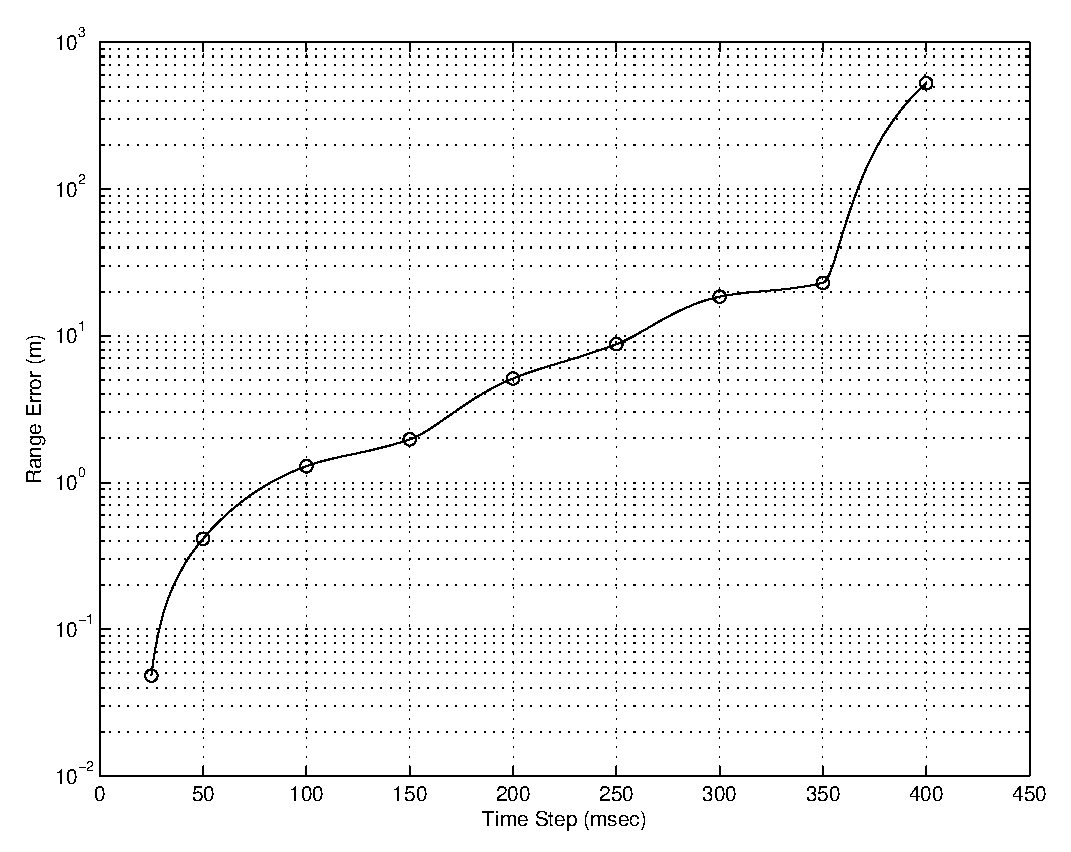
\includegraphics[width=3in]{refraction_pedersen_sensitivity.eps}} 
	\vspace*{8pt}
	\caption{Ray path accuracy as a function of step size 
		for the Pedersen/Gordon profile. 
	\label{fig:refraction_pedersen_sensitivity}}
\end{figure}
The sensitivity of these results to time step size is illustrated in
Fig.~\ref{fig:refraction_pedersen_sensitivity}. The 150~ms step size had
errors of about 2 meters. Errors for smaller time steps approached zero as
expected. Larger time steps increase as a power law until the step size was
larger than 350 ms, where the error quickly grew to hundreds of meters.
This sudden change in error appears to be the result of an inability of
model to properly sample the sound velocity profile field at the larger
step sizes. From this, we conclude that our earlier 100~ms time step
recommendation continues to be valid for this case.

\subsection{Ray path accuracy along great circle routes}

In this test, an ocean with a small amount of downward refraction was used
to verify the WaveQ3D model's ability to propagate rays along great circle
routes. Acoustic rays traveling at a constant depth follow these paths
because they are the shortest distance between two points along the
earth's surface. The amount of downward refraction needed to parallel the
earth's surface was computed by inverting Eq.~\ref{eq:cflat_adjustment}
\begin{equation}
	c(r) = \frac{r}{R} c_0  \:.
	\label{eq:chorizontal}
\end{equation}
where \(c_0\) was set to 1500~m/s. 

\begin{figure}[th]
	\centerline{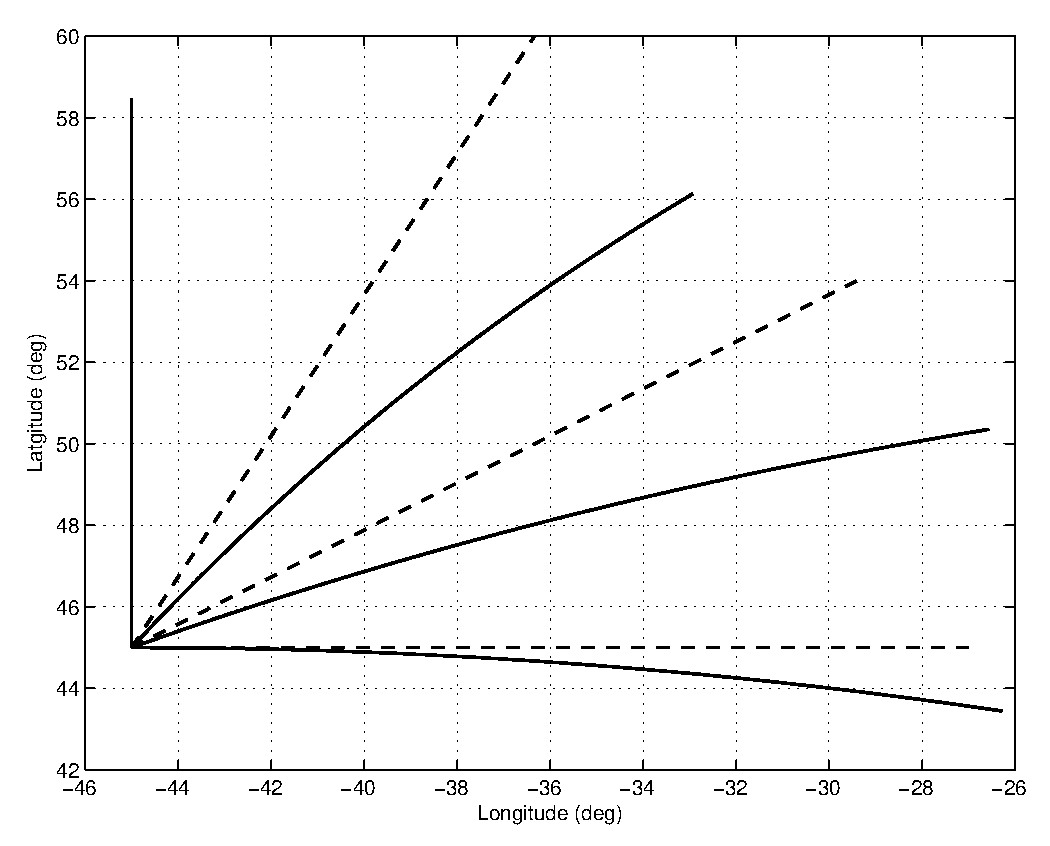
\includegraphics[width=3in]{refraction_great_circle.eps}} 
	\vspace*{8pt}
	\caption{Great circle routes. 
	\label{fig:gcroutes}}
\end{figure}
This test launched four horizontal rays from 45N 45W, at a depth of 1000
meters, with azimuths of 0\textsuperscript{o}, 30\textsuperscript{o},
60\textsuperscript{o}, and 90\textsuperscript{o}. The rays propagated for
1000~s (about 1500~km) with a time step of 100~ms.
Fig.~\ref{fig:gcroutes} illustrates the resulting ray paths as a function
of latitude and longitude. The solid lines represent acoustic ray paths
while the dashed lines represent the rhumb line paths, paths that would
have been taken if latitude/longitude were a Cartesian system. The accuracy
of the great circle routes were computed by converting the latitude,
longitude, and altitude of each ray back into a great circle azimuth at the
point of origin\cite{Williams2011}
\begin{equation}
	\varphi_a(t) = arctan \left[
		\frac{  \cos{\chi(t)} \sin(\phi(0)-\phi(t))}{ \cos{\chi(0)} \sin{\chi(t)}
		- \sin{\chi(0)} \cos{\chi(t)} \cos(\phi(0)-\phi(t)) } \right] \:,
	\label{eq:gc_bearing}
\end{equation}
where
\(\chi(t), \phi(t)\) are latitude and longitude as a function of time; and 
\(\varphi_a(t)\) is the analytic solution for the azimuthal launch angle
for a target at \(\chi(t), \phi(t)\).
The rays traveled at constant depth with a maximum deviation
from \(\varphi_a(t)\) of 2.81x10\textsuperscript{-10} degrees. This level of accuracy should be more than adequate for most applications.

\section{Interface Reflection Tests}

The WaveQ3D model estimates the partial time step during a 3-D interface
collision using the equation
\begin{equation}
	\delta t = \cfrac{h \: \hat{r} \cdot \hat{s}}{\cfrac{d\vec{r}}{dt} \cdot \hat{s}}
	\label{eq:reflection_time_bottom}
\end{equation}
where
\(\hat{s}\) is the surface normal;
\(\hat{r}\) is the unit vector in the radial direction;
$h$ is the incident ray height above bottom;
\(\delta t\) is the time step needed to reach the interface; and
\(\frac{dr}{dt}\) is the radial ray tracing component defined by Eq.~(\ref{eq:dr_dt}).
The direction of the 3--D reflection is computed using
\begin{equation}
	\hat{R} =  \hat{I} - 2 ( \hat{I} \cdot \hat{s} ) \hat{s}
	\label{eq:reflect_direction}
\end{equation}
where
\(\hat{I}\) is the incident ray path direction; and
\(\hat{R}\) is the reflected ray path direction.
The WaveQ3D model also applies a second order Taylor expansion to each
component of the position, normalized direction, and sound speed to improve
the accuracy of their values at the time of collision. The tests discussed
in this section analyze the accuracy of this reflection process in an
isovelocity ocean.

\subsection{Reflection accuracy with a flat bottom}

This test constructed a geometry in which the changes in latitude and travel
time for multiple interface bounces could be calculated analytically. The
path of a downwardly steered ray, given a constant bottom depth and
latitude change, is illustrated by Fig.~\ref{fig:reflect_flat_geo} and the equations
\begin{figure}[th]
	\centerline{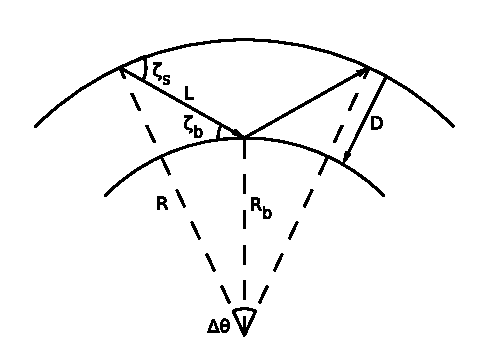
\includegraphics[width=3in]{ReflectFlat.eps}} 
	\vspace*{8pt}
	\caption{Flat bottom reflection geometry.  
	\label{fig:reflect_flat_geo}}
\end{figure}
\begin{equation}
	\zeta_s = arcsin \left( \frac{ R^2 - R_b^2 + L^2 }{ 2 R L } \right) \:,
	\label{eq:reflection_flat_sgrazing}
\end{equation}
\begin{equation}
	\zeta_b  = \zeta_s - \Delta\theta / 2 \:,
	\label{eq:reflection_flat_bgrazing}
\end{equation}
\begin{equation}
	t = L / c \:,
	\label{eq:reflection_flat_grazing}
\end{equation}
where
$R$ is the radius for the ocean surface;
$D$ is the water depth;
\( R_b = R - D \) is the radius for the ocean bottom;
\( \Delta\theta \) is the latitude change between surface bounces;
$L$ is the path length from surface to bottom;
\( \zeta_s \) is the grazing angle at the surface (also the ray launch angle);
\( \zeta_b  \) is the grazing angle at bottom;
$c$ is the sound speed; and
$t$ is the travel time between the surface and the bottom.

\begin{table}[th]
	\tbl{Flat bottom expected values.
	\label{tab:flat_reflect_test}}
	{\begin{tabular}{@{}cccc@{}} \toprule
		Parameter & Analytic Result \\ \colrule
		\( c \) & 1500~m/s \\
		\( D \) & 1000~m \\
		\( \Delta \theta \) & 0.2\textsuperscript{o} \\
		\( \zeta_s \) & 5.183617057\textsuperscript{o} \\
		\( \zeta_b \) & 5.083617057\textsuperscript{o} \\
		\( L \) & 11,175.841460125~m \\
		\( t \) & 7.450560973~s \\ \botrule
	\end{tabular}}
\end{table}
\( \Delta\theta \) was set 0.2\textsuperscript{o} and the ocean depth was
set to 1000 meters, which caused the remaining parameters take on the
analytic values shown in Table~\ref{tab:flat_reflect_test}. A single
WaveQ3D ray was launched at a depression/elevation angle of
-5.183617057\textsuperscript{o} (down), and a time step of 100~ms, which
produced the path shown in Fig.~\ref{fig:reflect_flat_test}. After four
complete cycles of bottom and surface reflection, a distance of about 89
km, the latitude for the point of reflection deviated from the analytic
result by less than 3.9x10\textsuperscript{-7} degrees (about 40~cm). The
travel time differed from the analytic result by less than
2.9x10\textsuperscript{-5}~s. From this, we conclude that the WaveQ3D
reflection process has an acceptable reflection accuracy when the
interfaces are flat.
\begin{figure}[th]
	\centerline{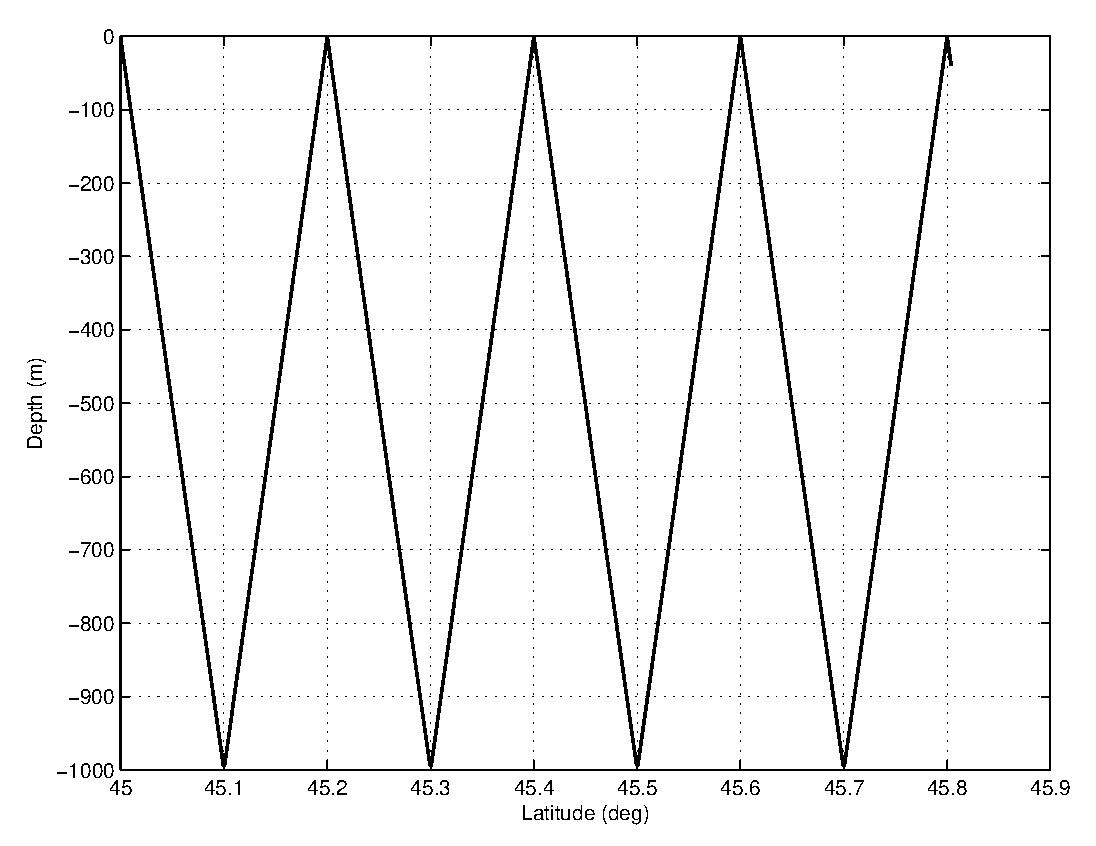
\includegraphics[width=3in]{reflect_flat_test.eps}} 
	\vspace*{8pt}
	\caption{Flat bottom reflection test results.  
	\label{fig:reflect_flat_test}}
\end{figure}

\subsection{Reflection accuracy with a sloped bottom}

This test looked at the ability of WaveQ3D to predict the direction of
reflection from a bottom that has a 1 degree up-slope in the latitude
direction. At each bottom reflection, the depression/elevation angle of the
WaveQ3D ray path should decrease by 2\textsuperscript{o}, just like the
analytic result. Launching a ray at a the same depression/elevation angle
as the last test (-5.183617057\textsuperscript{o}, down) produced the
results shown in Fig.~\ref{fig:reflect_slope_test}. Note that the time step
for this test was set to 1~ms to make it easier to compute
depression/elevation angle just before, and just after, each collision. The
maximum deviation of any of the three bottom reflections from their
analytic reflection direction result was 1x10\textsuperscript{-5} degrees.
From this, we conclude that WaveQ3D produces acceptable reflections for
sloped bottoms.
\begin{figure}[th]
	\centerline{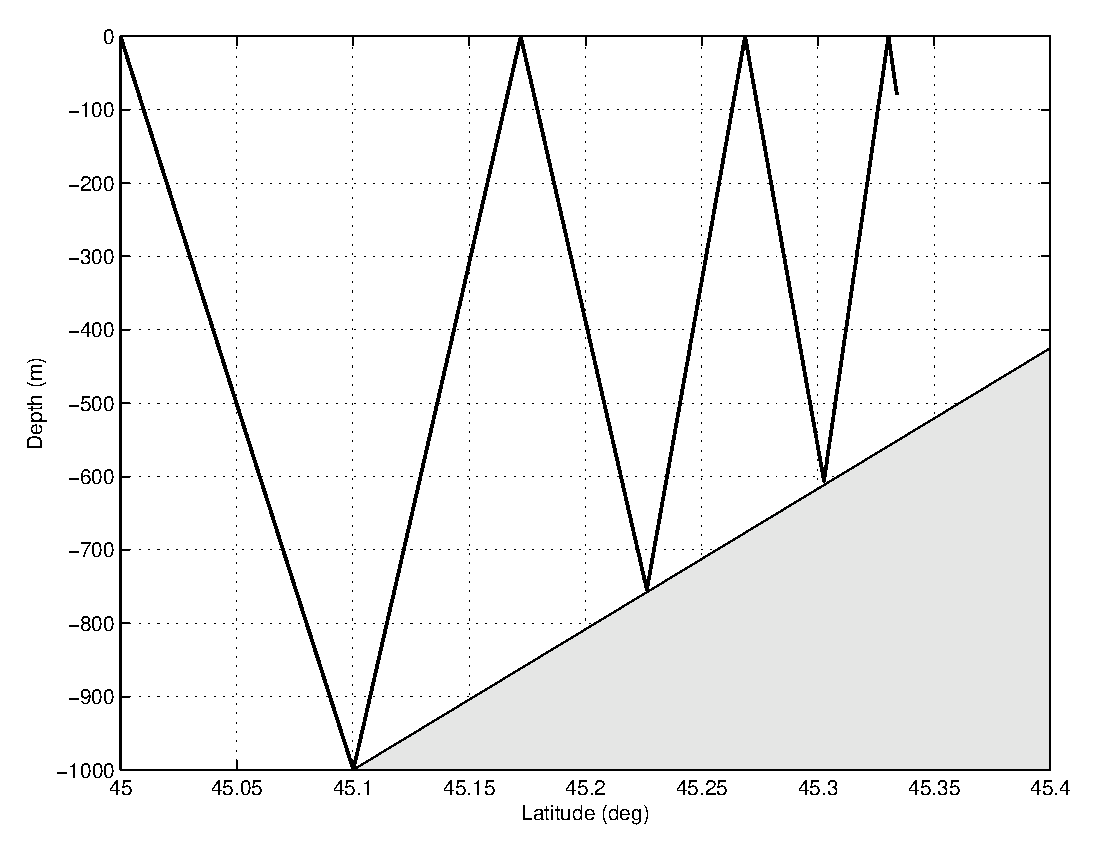
\includegraphics[width=3in]{reflect_slope_test.eps}} 
	\vspace*{8pt}
	\caption{Analytic slope reflection test results. 
	\label{fig:reflect_slope_test}}
\end{figure}

\subsection{Out-of-plane reflection from gridded bathymetry}

ETOPO1 gridded bathymetry\cite{ETOPO1} from the Malta Escarpment was used
to qualitatively test out-of-plane reflection from realistic bathymetry
features. Out-of-plane reflection is a real-world phenomena that can have a
significant impact on shallow water experiments.\cite{Sturm2008} To isolate
the testing to reflection effects, the speed of sound was fixed at 1500~m/s
at all locations. WaveQ3D used a 100~ms step size to compute a single path,
illustrated in Figure~\ref{fig:reflect_grid_malta}. In this figure, bottom
bathymetry contours are represented as dashed lines. A ray launched from
35:59N 16:00E, at a depth of 10 meters, with a depression/elevation angle
of -20\textsuperscript{o} (down), and an azimuth of 270\textsuperscript{o}
traveled along the path illustrated by the solid black line. The closed
circles along this path represent places where bottom reflections occurred;
the open circles represent surface reflections. The decrease in spacing
between the shallow water dots illustrates the type of depression/elevation
angle change (Fig.~\ref{fig:reflect_slope_test}) expected for sloped
bottoms. What was new in this test was the face that ray paths were
reflected into a new azimuthal direction each time that they interacted
with the bottom. These out-of-plane reflections resulted in a down slope
ray path that was offset by more than 21.9 km from the up slope path, after
14 bounces off of the bottom. From this, we conclude that WaveQ3D results
will have a significant contributions from out-of-plane ray paths whenever
there are multiple interactions with complex bottom bathymetry features.
\begin{figure}[th]
	\centerline{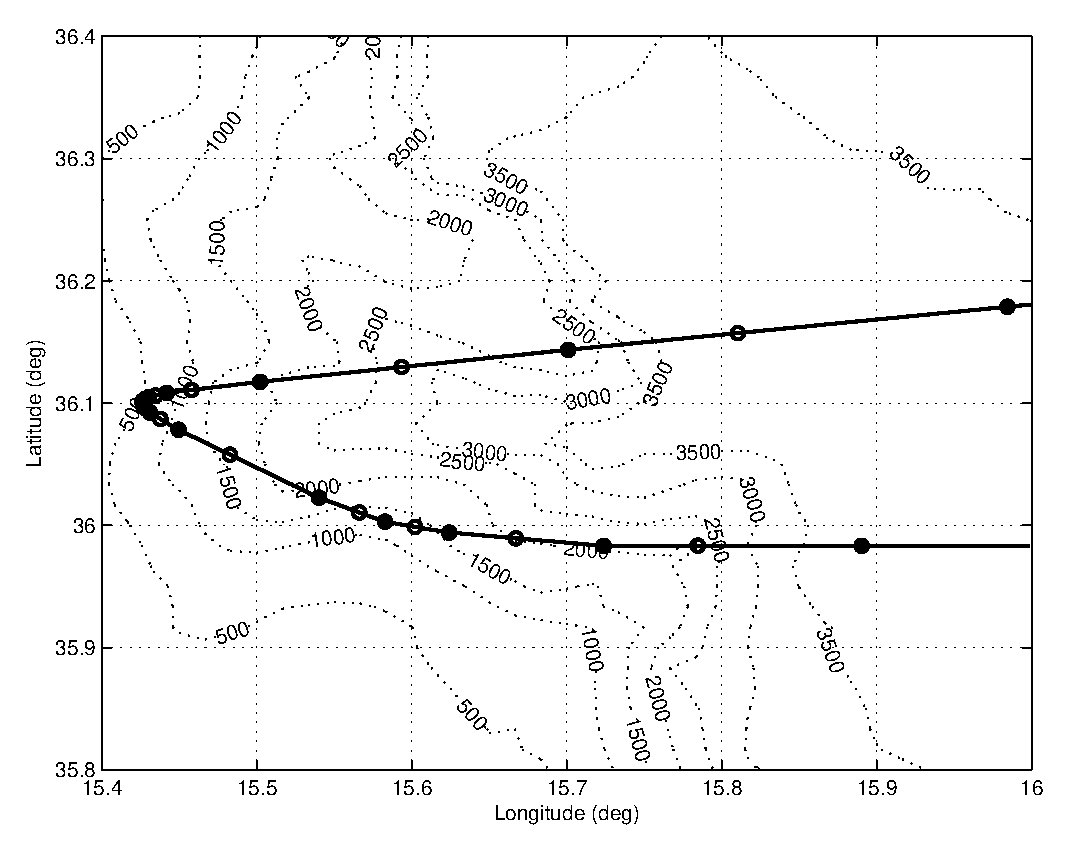
\includegraphics[width=3in]{reflect_grid_malta.eps}} 
	\vspace*{8pt}
	\caption{Reflection on the Malta Escarpment.
	\label{fig:reflect_grid_malta}}
\end{figure}

\section{Eigenray and Propagation Loss Tests}

The tests discussed in this section compare WaveQ3D's eigenray and propagation
loss calculation to analytic solutions.

The WaveQ3D eigenray estimation process establishes the relative geometry
between rays paths and targets. That geometry then allows the calculation
of travel time ($t$), source angle (\(\mu\)), and target angle
(\(\varphi\)) for each multi-path arrival. WaveQ3D computes these eigenray
products by searching for the offsets which minimize the squared distance
from targets to points on the wavefront. Once the CPA has been determined,
the 3-D offset to the target is computed using
\begin{equation}
	\vec{\rho} \equiv (\rho_1, \rho_2, \rho_3) 
		\equiv (\delta t, \delta \mu, \delta \varphi) \:,
	\label{eq:rho_defined}
\end{equation}
\begin{equation}
	\vec{g} \equiv \frac{\partial d^2}{\partial \vec{\rho} } \big|_{CPA} \:,
	\label{eq:taylor3}
\end{equation}
\begin{equation}
	\mathbf{H} \equiv \frac{\partial^2 d^2}{\partial \vec{\rho}^2 } \big|_{CPA}
	\label{eq:taylor4}
\end{equation}
\begin{equation}
	\vec{\rho} = - \mathbf{H}^{-1} \: \vec{g} \:.
	\label{eq:inverse3}
\end{equation}
where 
\(\vec{\rho}\) is the offset from CPA in vector form;
\(d^2\) is the squared distance from each point on the wavefront to the target;
\(\vec{g}\) is the gradient of squared distance, evaluated at CPA (3 elements), and
\(\mathbf{H}\) is the Hessian matrix of squared distance, evaluated at CPA (3x3).

The propagation loss at the target location is a summation of
contributions from the rays that surround the eigenray target. 
To create a 3-D acoustic field across the wavefront, WaveQ3D uses 
independent Gaussian beams in the
\(\mu\) and \(\varphi\) directions and ignores the cross terms. 
\begin{equation}
	G(\vec{r}_p) = \left( \sum_{j'=j-J}^{j+J} g_{j'}(\vec{r}_p)\right) 
		\left( \sum_{k'=k-K}^{k+K} g_{k'}(\vec{r}_p)\right) \:,
	\label{eq:gaussian_sum}
\end{equation}
\begin{equation}
	g_{j'}(\vec{r}_p) = \frac{ \left( \mu_{j'+1} - \mu_{j'} \right) }
		{\sqrt{2\pi w^2_{j'}}} 
		\: exp \left( - \frac{d^2_{j'}}{2w^2_{j'}} \right) \:,
	\label{eq:gaussian_each1}
\end{equation}
\begin{equation}
	g_{k'}(\vec{r}_p) = \frac{ \left( sin(\mu_{j'+1}) - sin(\mu_{j'}) \right) 
		\left( \varphi_{k'+1} - \varphi_{k'} \right) }
		{\sqrt{2\pi w^2_{k'}}} 
		\: exp \left( - \frac{d^2_{k'}}{2w^2_{k'}} \right) \:,
	\label{eq:gaussian_each2}
\end{equation}
where
\(G(\vec{r}_p)\) is the total Gaussian beam intensity at the eigenray target;
$(j,k)$ are the index numbers of wavefront cell containing the eigenray target;
\(g_{j'}\) are the Gaussian beam contributions along depression/elevation direction;
\(g_{k'}\) are the Gaussian beam contributions along the azimuthal direction;
$2J+1$ are the number of significant beams in the depression/elevation direction; and
$2K+1$ are the number of significant beams in the azimuthal direction;
\(w_j\) and \(w_k\) are the half-widths of the Gaussian beam in the \(\mu\)
and \(\varphi\) directions; and
\(d^2_{j}\) and \(d^2_{k}\) are the distance in the \(\mu\) and \(\varphi\)
directions from the Gaussian beam center to the eigenray target. The WaveQ3D
implementation divides the wavefront into ray families based on the number
of surface reflections, bottom reflections, and caustic encounters. Within
each ray family, propagation loss contributions are added across the
wavefront until an edge is hit or the accumulated loss result changes by
less than 0.01 dB.

WaveQ3D treats the beam width calculation as a convolution between Weinberg's
frequency dependent ``minimum width'' term\cite{Weinberg1996} and a second
Gaussian that represents the spatial spreading created by the sampling of
the wavefront.
\begin{equation}
	(w'_{j,k}(f))^2 = \left( 2 w_{j,k} \right)^2 + \left( 2 \pi \lambda \right)^2 \:.
	\label{eq:new_width}
\end{equation}
where
\(\lambda\) is the wavelength of the signal being modeled;
\(w_{j,k}\) is the cell width of beam $j$ or $k$, and
\(w'_{j,k}(f)\) is the adjusted width of beam $j$ or $k$.
The factor of 2 in the \(w_{j,k}\) term creates a minimum overlap of 50\%
between neighboring beams. Normalizing Eqs.~(\ref{eq:gaussian_each1}) and
(\ref{eq:gaussian_each2}) by the combined effect of both spreading sources
conserves energy across the wavefront.

\subsection{Eigenray accuracy for a simple geometry}

This test constructs a short range geometry in which travel time, source
angle, and target angle can be computed analytically for direct path,
surface reflected, and bottom reflected paths on a spherical earth. The
geometry for this test is illustrated in Fig.~\ref{fig:eigenray_basic}.
\begin{figure}[th]
	\centerline{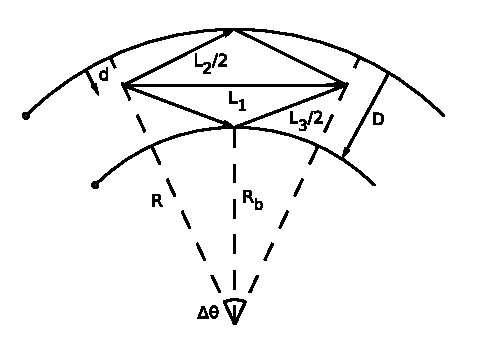
\includegraphics[width=3in]{EigenrayBasic.eps}} 
	\vspace*{8pt}
	\caption{Flat bottom eigenray test geometry. 
	\label{fig:eigenray_basic}}
\end{figure}
\begin{equation}
	r = R - d \:,
	\label{eq:eigenray_flat_h}
\end{equation}
\begin{equation}
	L_1 = 2 r sin( \Delta \theta / 2 ) \:,
	\label{eq:eigenray_flat_L1}
\end{equation}
\begin{equation}
	\mu_1 = 90^o - arccos \left( \frac{L_1}{2r} \right) \:,
	\label{eq:eigenray_flat_mu1}
\end{equation}
\begin{equation}
	L_2 = 2 \sqrt{ (L_1/2)^2 + [R-r \: cos(\Delta \theta / 2)]^2 } \:,
	\label{eq:eigenray_flat_L2}
\end{equation}
\begin{equation}
	\mu_2 = 90^o - arccos \left( \frac{d}{L_2/2} \right) \:,
	\label{eq:eigenray_flat_mu2}
\end{equation}
\begin{equation}
	L_3 = 2 \sqrt{ (L_1/2)^2 + [r \: cos(\Delta \theta / 2) - (R-D)]^2 } \:,
	\label{eq:eigenray_flat_L3}
\end{equation}
\begin{equation}
	\mu_3 = \mu_1 + arccos \left( \frac{L_1/2}{L_3/2} \right) \:,
	\label{eq:eigenray_flat_mu3}
\end{equation}
\begin{equation}
	t_n = L_n / c \:,
	\label{eq:eigenray_flat_c}
\end{equation}
where
$c$ is the sound speed;
$D$ is the water depth;
$d$ is both the source and target depth;
$r$ is the distance of the source/target from the center of curvature; 
\( L_1, L_2, L_3 \) are the path lengths for the direct, surface reflected,
and bottom reflected paths;
\( t_1, t_2, t_3 \) are the travel times; and
\( \mu_1, \mu_2, \mu_3 \) are the source/target depression/elevation angles.

WaveQ3D was tested using an ocean depth of 3000 m, a \( \Delta\theta \) value of 0.02\textsuperscript{o}, and the source/target depth of 1000 m.  Eqs. (\ref{eq:eigenray_flat_h}) through (\ref{eq:eigenray_flat_c}) were then used to compute the values shown in
Table~\ref{tab:flat_eigenray_test}.

\begin{table}[th]
	\tbl{Expected eigenray values for a simple geometry.
	\label{tab:flat_eigenray_test}}
	{\begin{tabular}{@{}cccc@{}} \toprule
		Parameter & Analytic Result \\ \colrule
		\( D \) & 3000~m \\
		\( d \) & 1000~m \\
		\( \Delta \theta \) & 0.02\textsuperscript{o} \\
		\( t_1 \) & 1.484019~s \\
		\( t_2 \) & 1.995103~s \\
		\( t_3 \) & 3.051677~s \\
		\( \mu_1 \) & -0.010000\textsuperscript{o} \\
		\( \mu_2 \) & 41.936232\textsuperscript{o} \\
		\( \mu_3 \) & -60.912572\textsuperscript{o} \\ \botrule
	\end{tabular}}
\end{table}

WaveQ3D eigenrays were calculated using a ray fan with
depression/elevation angles from -60\textsuperscript{o} to
+60\textsuperscript{o}, azimuth angles from -4\textsuperscript{o} to
+4\textsuperscript{o}, angle spacings of 1\textsuperscript{o} in both
directions, and a time step of 100~ms. This geometry was
specifically designed to stress the model by forcing it to extrapolate the
bottom bounce path from a location outside of the ray fan. The other two
paths are firmly inside of the ray fan.

For the direct path, the maximum difference between the modeled
times/angles and their analytic counterparts were
2.2x10\textsuperscript{-5}~ms and 1.1x10\textsuperscript{-4} degrees. These
values represented eigenray accuracy limitations purely derived from
Eqs.~(\ref{eq:rho_defined}) through (\ref{eq:inverse3}). The equivalent
measurements for the surface reflected path yielded differences of
2.2x10\textsuperscript{-3}~ms and 4.8x10\textsuperscript{-3} degrees. The
reduced accuracy of the surface reflected paths appears to be due to
limitations in the interface reflection process. Even thought the bottom
reflected path was extrapolated from outside of the ray fan, it still
achieved accuracies of 1.7~ms and 0.91\textsuperscript{o}. We believe that
any of these eigneray accuracies should be adequate for most sim/stim
applications.

\subsection{Eigenray accuracy for Lloyd's mirror on spherical earth} 

On a flat earth, the Lloyd's mirror geometry generates exactly two paths: a
direct path and a surface reflection. However (as shown in
Fig.~\ref{fig:eigenray_concave_rays1}) isovelocity ray paths actually form
unexpected caustics when the curvature of the earth is incorporated.
Fig.~\ref{fig:eigenray_concave_rays2} illustrates that these caustics are
formed by focusing from the concave surface of the earth. Incorporating
these effects into our eigneray tests is important because of WaveQ3D's use
of spherical earth coordinates.
\begin{figure}[th]
	\centerline{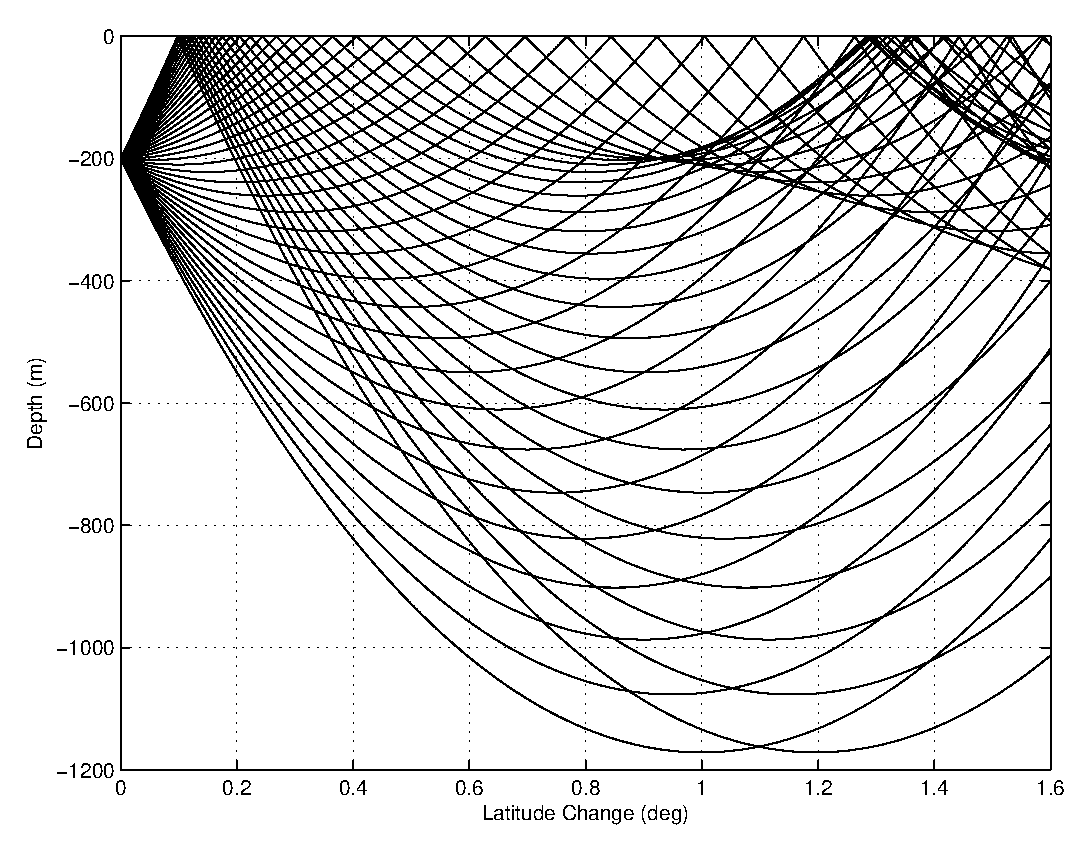
\includegraphics[width=3in]{eigenray_concave_rays1.eps}} 
	\vspace*{8pt}
	\caption{Isovelocity paths in spherical coordinates. 
	\label{fig:eigenray_concave_rays1}}
\end{figure}
\begin{figure}[th]
	\centerline{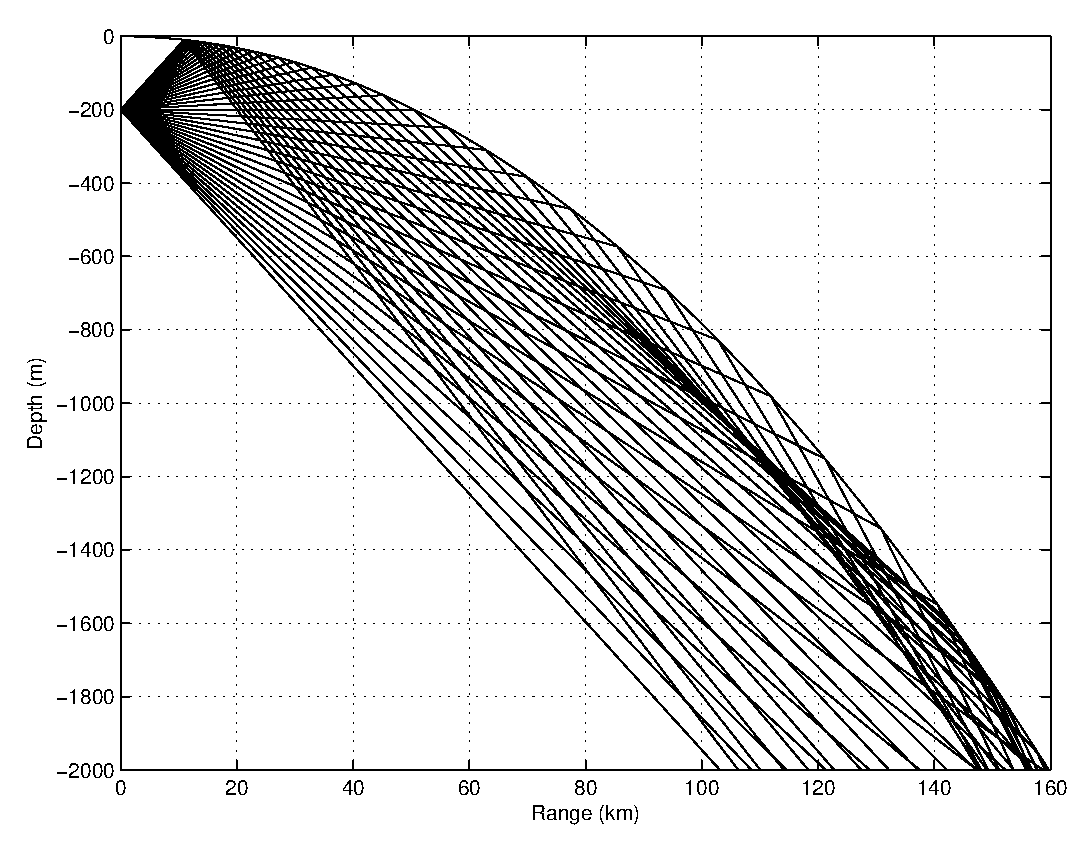
\includegraphics[width=3in]{eigenray_concave_rays2.eps}} 
	\vspace*{8pt}
	\caption{Isovelocity paths in Cartesian coordinates. 
	\label{fig:eigenray_concave_rays2}}
\end{figure}

Fig.~\ref{fig:eigenray_lloyds} defines the geometry used to compute an
analytic eigenray solution.  In this figure,
\( d_1, d_2 \) are the source and target depths; 
\( r_1, r_2 \) are the source and target distance from the center of curvature; 
\( \Delta \theta \) is the latitude change from source to target;
\( \Delta \theta_1 \) is the latitude change from the source to the point of reflection;
\( \Delta \theta_2 = \Delta \theta - \Delta \theta_1 \) is the latitude change from the reflection point to the target;
\( \beta \) is the reflection angle relative to the normal;
$a$ is the length of the direct path; and
\( b_1 + b_2 \) is the length of the surface reflected path.
\begin{figure}[th]
	\centerline{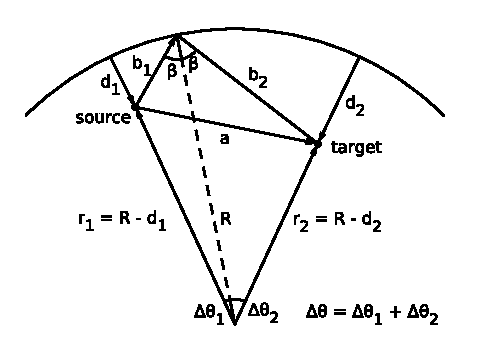
\includegraphics[width=3.5in]{EigenrayLloyds.eps}} 
	\vspace*{8pt}
	\caption{Ocean surface as concave reflector.
	\label{fig:eigenray_lloyds}}
\end{figure}

The analytic solutions for the surface reflected path requires finding
values of \( \Delta \theta_1 \) which solve the transcendental equation
(derived in the Appendix A)
\begin{equation}
	r_1 sin( \Delta \theta_1 ) - r_2 sin( \Delta \theta - \Delta \theta_1 ) 
		+ \frac{r_1 r_2}{R} sin( \Delta \theta - 2 \Delta \theta_1 ) = 0 \:.
	\label{eq:surf_reflected}
\end{equation}
Once the roots of Eq.~(\ref{eq:surf_reflected}) are known, the analytic
solution for surface reflected eigenrays can be computed using
\begin{equation}
	b_1^2 = R^2 + r_1^2 - 2 R r_1 \: cos( \Delta \theta_1 ) \:,
	\label{eq:eigenray_lloyds_a1}
\end{equation}
\begin{equation}
	b_2^2 = R^2 + r_2^2 - 2 R r_2 \: cos( \Delta \theta_2 ) \:,
	\label{eigenray_lloyds_analyticeq:eigenray_lloyds_a2}
\end{equation}
\begin{equation}
	t_s = \frac{ b_1 + b_2 }{c_0} \:,
	\label{eq:eigenray_lloyds_tsurface}
\end{equation}
\begin{equation}
	\mu_{s,source} = - arcsin \left( \frac{b_1^2+r_1^2-R^2}{2 b_1 r_1} \right) \:,
	\label{eq:eigenray_lloyds_eta1}
\end{equation}
\begin{equation}
	\mu_{s,target} = arcsin \left( \frac{b_2^2+r_2^2-R^2}{2 b_2 r_2} \right) \:,
	\label{eq:eigenray_lloyds_eta2}
\end{equation}
where
\( t_s \) is the surface-reflected travel time from source to target;
\( \mu_{s,source} \) is the surface-reflected depression/elevation angle at source; and
\( \mu_{s,target} \) is the surface-reflected depression/elevation angle at target.

\begin{figure}[th]
	\centerline{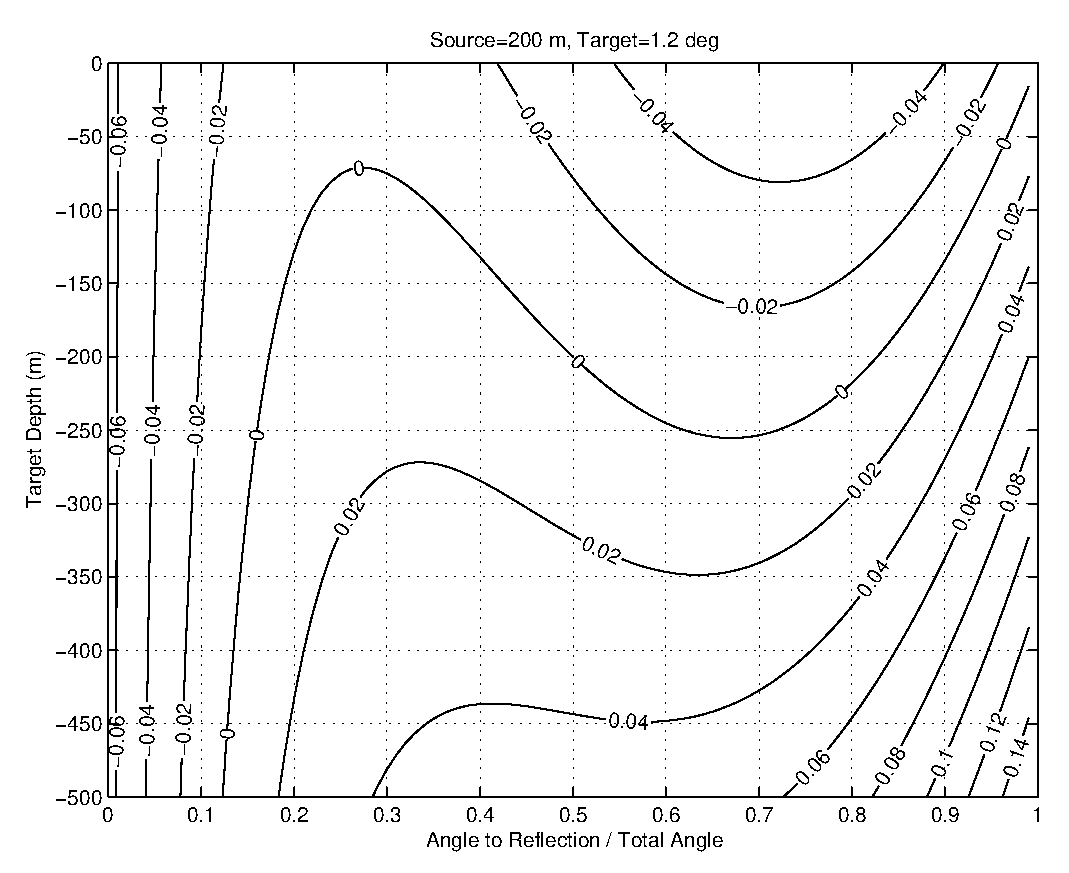
\includegraphics[width=3in]{eigenray_lloyds_analytic.eps}} 
	\vspace*{8pt}
	\caption{Roots of surface reflection transcendental equation.  
	\label{fig:eigenray_lloyds_analytic}}
\end{figure}
Fig.~\ref{fig:eigenray_lloyds_analytic} illustrates the roots of
Eq.~(\ref{eq:surf_reflected}) for a source depth of 200 meters. The horizontal
axis is the ratio of \(\Delta \theta_1 / \Delta \theta \). The vertical
axis defines target depths from 0 to 500 meters. The contours on this plot
represent the values for the left hand side of
Eq.~(\ref{eq:surf_reflected}), multiplied by 10\textsuperscript{5}, for a target
\(\Delta \theta\) of 1.2\textsuperscript{o}. The zero contour illustrates
the location of the roots at each target depth. For example, we found that
there are three roots for \(\Delta \theta_1\) at values of \(\Delta
\theta\) times 0.190047203712437, 0.425088688451783, and 0.88486312787168
when a target depth was 150 meters. The physical interpretation of the
multiple roots is that there are multiple surface-reflection paths focused
onto the target location by the concave surface of the earth.

\begin{table}[th]
	\tbl{Expected eigenray values for target at 1.2\textsuperscript{o} and 150 m.
	\label{tab:eigenray_concave}}
	{\begin{tabular}{@{}lccc@{}} \toprule
		Path & Travel time& Launch angle & Target angle\\ \colrule
		Direct Path & 89.05102557~s & -0.578554378\textsuperscript{o} 
			& +0.621445622\textsuperscript{o} \\
		Surface 1 & 89.05369537~s & +0.337347599\textsuperscript{o} 
			& +0.406539112\textsuperscript{o} \\
		Surface 2 & 89.05379297~s & -0.053251329\textsuperscript{o} 
			& +0.233038477\textsuperscript{o} \\
		Surface 3 & 89.05320459~s & -0.433973977\textsuperscript{o} 
			& -0.48969753\textsuperscript{o} \\  \botrule
	\end{tabular}}
\end{table}

The analytic eigenray products for a target at a depth of 150 m are shown
in Table~\ref{tab:eigenray_concave}. WaveQ3D was run with a time step of
100~ms and a depression/elevation launch angle spacing of
0.05\textsuperscript{o}. The travel times computed by WaveQ3D matched the
analytic result to within 1.2x10\textsuperscript{-5}~s, and the angles were
accurate to within 0.012\textsuperscript{o}. Note that rhe launch angle
spacing was much tighter than other tests because WaveQ3D's eigenray
searching logic is limited to finding one ray path between any two launch
angles. A larger launch angle increment in this test would have caused the
model to fail to find the "Surface 3" path. But with this context, we felt
that WaveQ3D was quite accurate in predicting the travel times and angles
for the equivalent of a Lloyd's mirror geometry on a spherical earth.

\subsection{Eigenray robustness for Lloyd's mirror on spherical earth}

This test extends the results of the previous section by comparing modeled
travel times and ray path angles, for the spherical equivalent of Lloyd's
mirror, at a variety of depths and ranges.
This test used a isovelocity speed of sound of 1500~m/s, a frequency of
2000~Hz, a source depth of 200 m, target depths from 0 to 1000 m, 181
tangent spaced depression/elevation angles (explained in the Appendix B),
1\textsuperscript{o} spaced azimuth angles from -4\textsuperscript{o} to
+4\textsuperscript{o}, and a time step of 100~ms. The maximum range was
limited to \(\Delta \theta = 0.8\textsuperscript{o}\) to ensure that only a
single surface reflected path was produced at each target location (see
Fig.~\ref{fig:eigenray_concave_rays1}). This choice allows the test to be
run with a ray spacing that was much more typical than the fine scale D/E
angles used in the previous section.
\begin{figure}[th]
	\centerline{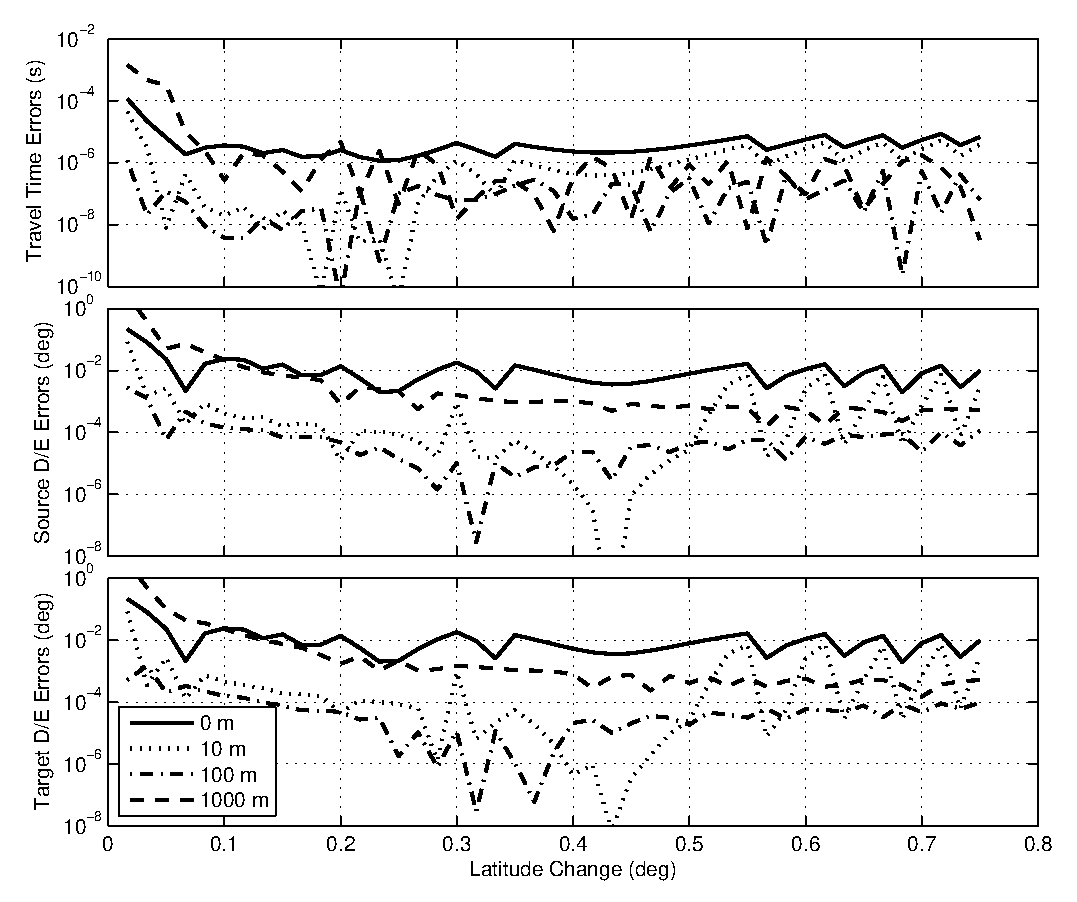
\includegraphics[width=4in]{eigenray_lloyds_0.eps}} 
	\vspace*{8pt}
	\caption{Eigenray errors for Lloyd's mirror direct path.
	\label{fig:eigenray_lloyds_0}}
\end{figure}

The eigenray errors for direct path are summarized in
Fig.~\ref{fig:eigenray_lloyds_0}. Each plot shows the absolute value of the
difference between the WaveQ3D model and the analytic solution, as a
function of range, for targets at depths of 0, 10, 100, and 1000 m. Beyond
a range of 0.1\textsuperscript{o} (about 11 km), the direct path model had
maximum errors in travel time error and angle of 0.0087~ms and
0.024\textsuperscript{o}. In each case, these errors were larger at short
ranges. The short range errors were most pronounced near the ocean surface
and at the 1000~m depth.

The eigenray errors for the surface reflected path are shown in
Fig.~\ref{fig:eigenray_lloyds_1}. Once again, the errors were largest at
short ranges, both near the ocean surface and at the 1000~m depth. Beyond a range of
0.1\textsuperscript{o}, the surface reflected path model has a maximum
travel time error of 0.0041~ms, a maximum source angle
error of 0.055\textsuperscript{o} and a maximum target angle error of
0.047\textsuperscript{o}. In each case, the errors are larger at short
ranges.
\begin{figure}[th]
	\centerline{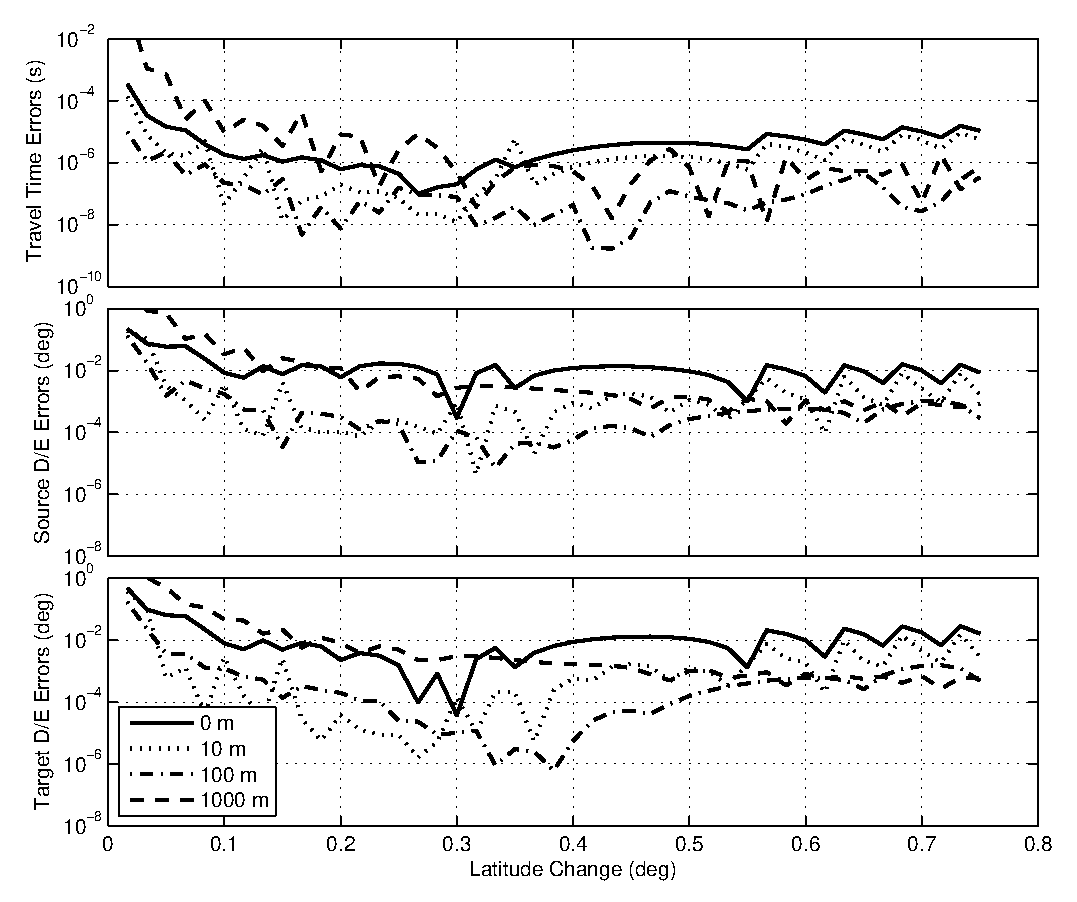
\includegraphics[width=4in]{eigenray_lloyds_1.eps}} 
	\vspace*{8pt}
	\caption{Eigenray errors for Lloyd's mirror surface reflected path.
	\label{fig:eigenray_lloyds_1}}
\end{figure}

The inaccuracies near the surface were attributed to undersampling by the
100~ms time step, as illustrated in Fig.~\ref{fig:eigenray_lloyds_zoom}.
The solid lines in this figure represent direct path rays that are moving
out in range and up toward the surface from the source at 200 m. The dashed
lines present the same ray paths after reflection from the ocean surface.
The dotted lines that connect them represent discontinuities between the
direct path and surface reflected segments of the wavefront. At short
ranges, these discontinuities cause the edges of ray families to be far
from targets that are near the interface; extrapolation led to inaccuracy.
Shortening the time step mitigates this source of inaccuracy. At longer
ranges, this source of inaccuracy is automatically reduced by the fact that
the edges of the ray families get closer to the surface as the rays become
more horizontal.
\begin{figure}[th]
	\centerline{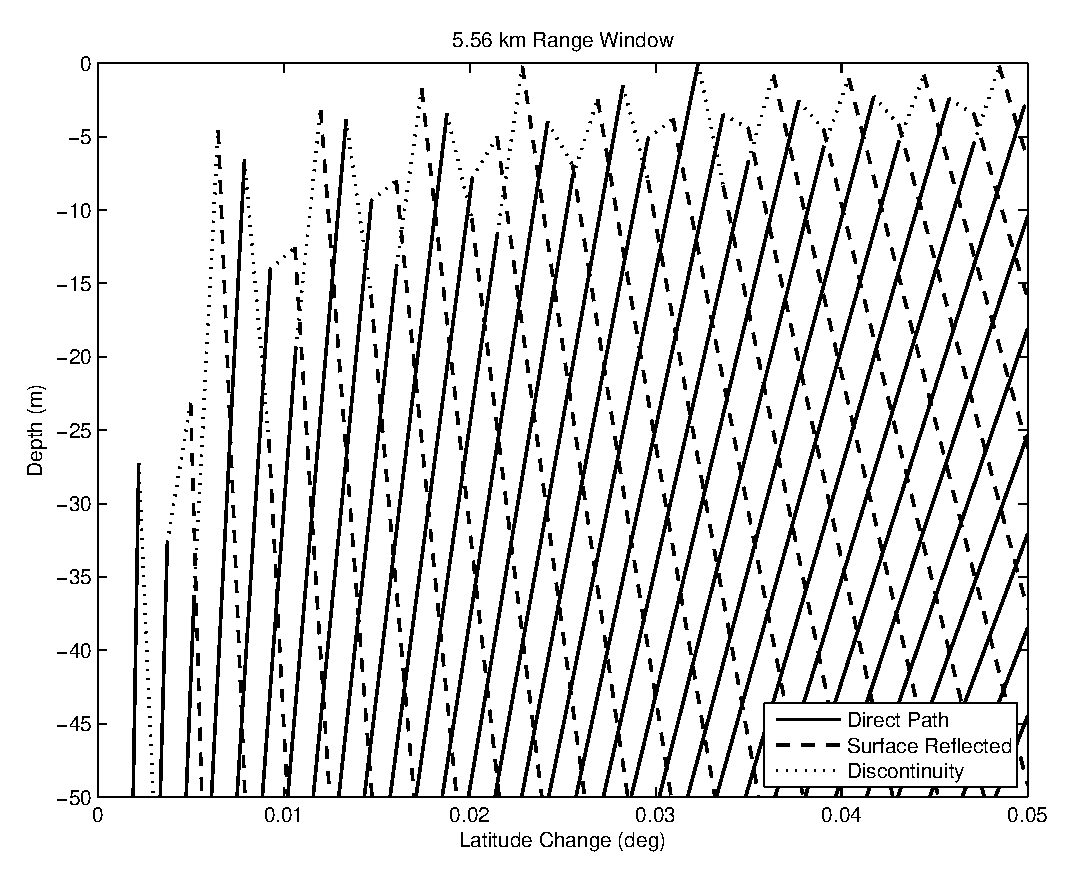
\includegraphics[width=3in]{eigenray_lloyds_zoom.eps}} 
	\vspace*{8pt}
	\caption{Time-step effects near the ocean surface.
	\label{fig:eigenray_lloyds_zoom}}
\end{figure}

The errors at large depths were attributed to the tangent spaced
depression/elevation angles used in this test. Using a more uniform scheme
for depression/elevation angles would have mitigated this source of
inaccuracy.

\subsection{Propagation loss accuracy for Lloyd's Mirror}

Near the surface, WaveQ3D must extrapolate eigenrays from distances that
are up to 1.5 paths away from the interface. The tests in this section were
designed to expose the impact of this limitations on propagation loss
accuracy. The analytic solutions for these test were derived in Cartesian
coordinates using the method of images.
\begin{equation}
	p(r,z) = \frac{ e^{ikL_1} }{ L_1 } - \frac{ e^{ikL_2} }{ L_2 } \:;
	\label{eq:lloyd_flat_p}
\end{equation}
\begin{equation}
	L_1 = \sqrt{ r^2 + ( z - z_s )^2 } \:;
	\label{eq:lloyd_flat_l1}
\end{equation}
\begin{equation}
	L_2 = \sqrt{ r^2 + ( z + z_s )^2 } \:;
	\label{eq:lloyd_flat_l2}
\end{equation}
where
$r$ is the target range;
$z$ is the target depth (positive is down);
\( z_s \) is the source depth (positive is down);
\( L_1 \) is the slant range to source;
\( L_2 \) is the slant range to image source (above water);
$k$ is the acoustic wave number (\( 2 \pi f / c \)); and
$f$ is the signal frequency;
$c$ is the speed of sound;
\( p(r,z) \) is the complex pressure.

The propagation loss for a 200 meters deep target is shown as a function of
range in Fig.~\ref{fig:proploss_lloyds_range} and
Fig.~\ref{fig:proploss_lloyds_range_zoom}. Results for a 10 km range target
are shown as a function of depth in Fig.~\ref{fig:proploss_lloyds_depth}.
Both cases used a speed of sound of 1500~m/s, with a ``flat earth''
adjustment from Eq. (\ref{eq:cflat_adjustment}), a frequency of 2000~Hz, a
source depth of 75~m, 181 tangent spaced depression/elevation angles,
1\textsuperscript{o} spaced azimuth angles from -4\textsuperscript{o} to
+4\textsuperscript{o}, and a time step of 100~ms.
Figure~\ref{fig:proploss_lloyds_range_zoom} highlights fact that the errors
in Fig.~\ref{fig:proploss_lloyds_range} are most sever at range less than 2
km. Figure~\ref{fig:proploss_lloyds_range_zoom} illustrates that fact that
the largest errors, as a function of depth, are right below the ocean
surface. We attribute the ocean surface results to small in the computation
of travel time for the direct and surface reflected paths.
\begin{figure}[th]
	\centerline{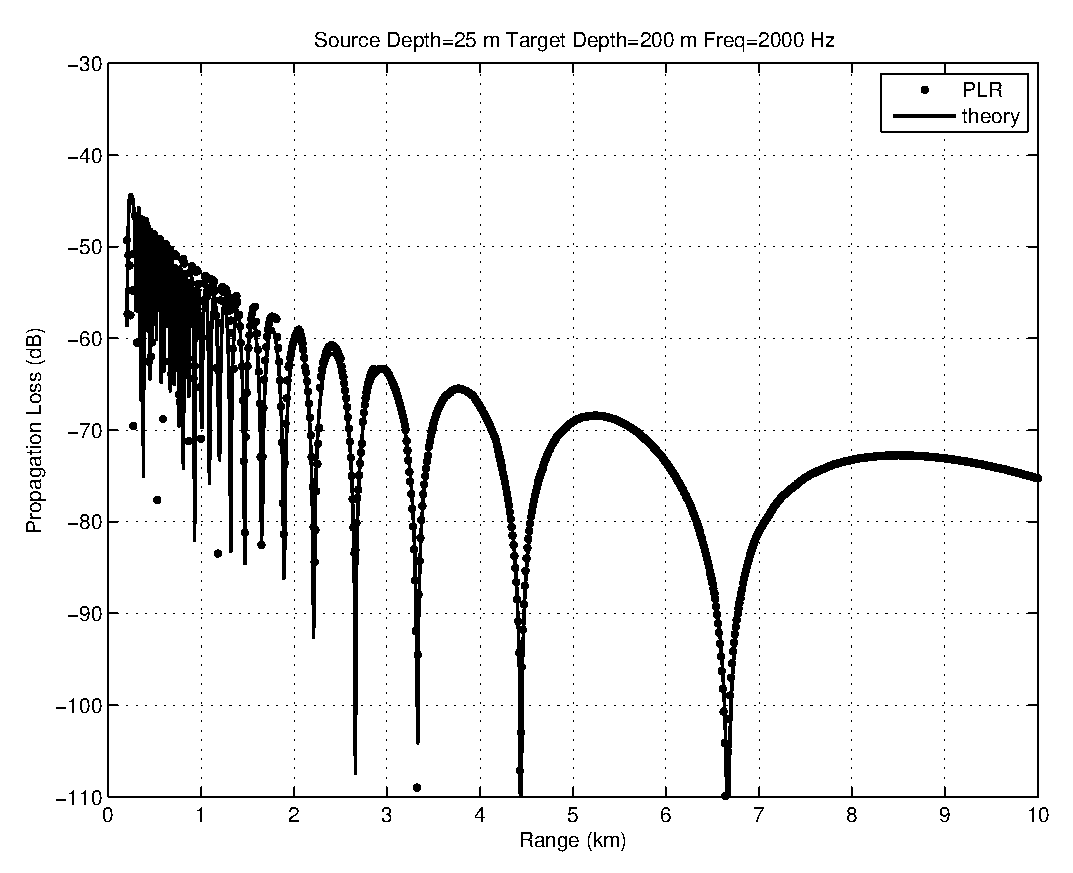
\includegraphics[width=3in]{proploss_lloyds_range.eps}} 
	\vspace*{8pt}
	\caption{Lloyd's mirror propagation loss as a function of range. 
	\label{fig:proploss_lloyds_range}}
\end{figure}
\begin{figure}[th]
	\centerline{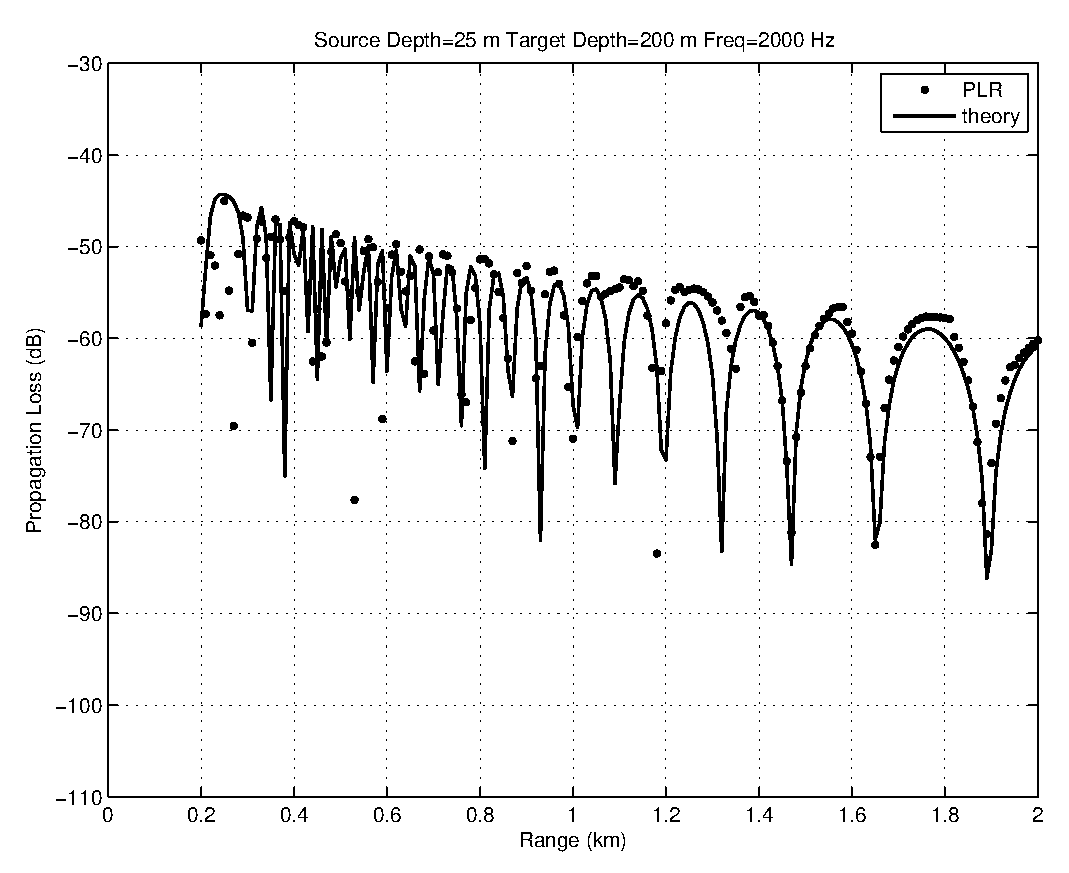
\includegraphics[width=3in]{proploss_lloyds_range_zoom.eps}} 
	\vspace*{8pt}
	\caption{Lloyd's mirror propagation loss errors at short ranges.
	\label{fig:proploss_lloyds_range_zoom}}
\end{figure}
\begin{figure}[th]
	\centerline{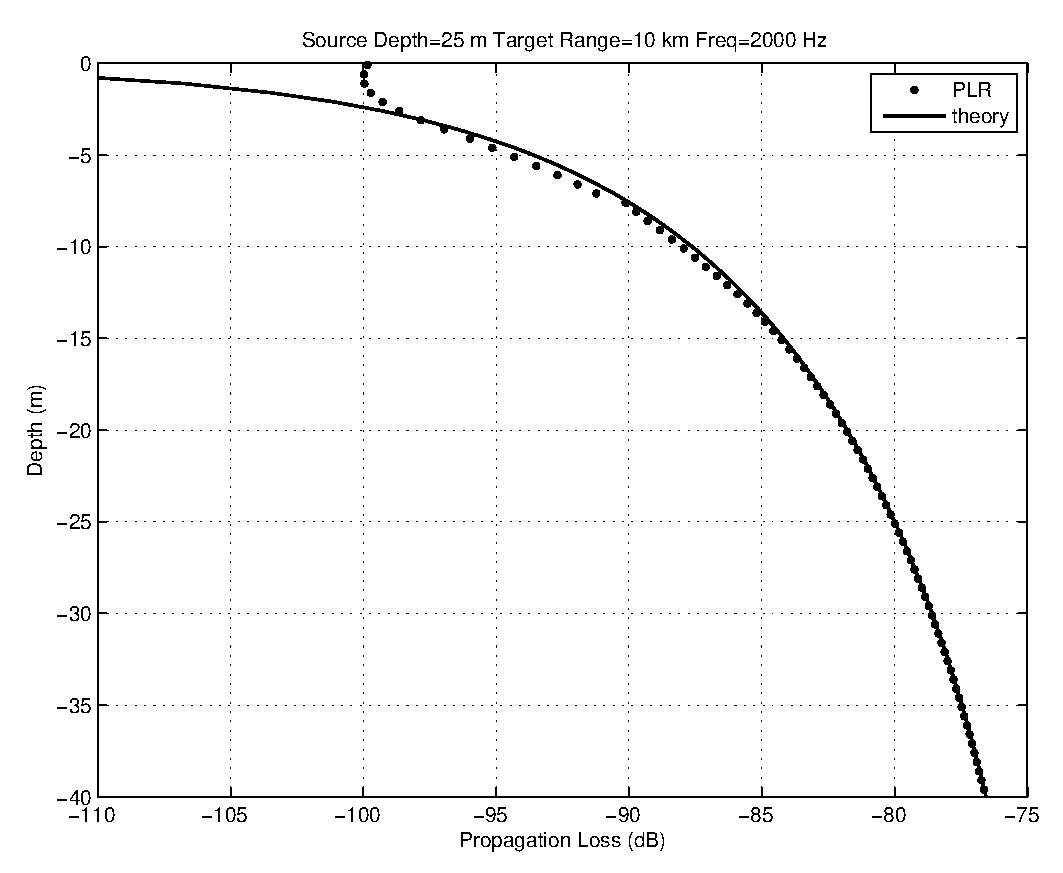
\includegraphics[width=3in]{proploss_lloyds_depth.eps}} 
	\vspace*{8pt}
	\caption{Lloyd's mirror propagation loss as a function of depth. 
	\label{fig:proploss_lloyds_depth}}
\end{figure}

To compare these results quantitatively, we will use a set of statistical
measures that are defined in detail in Appendix C. The differences between
the WaveQ3D model and the analytic results are summarized in
Table~\ref{tab:proploss_lloyds_accuracy}. From this, we conclude that,
although the WaveQ3D model's Lloyd's Mirror predictions clearly has
limitations, those limitations will have a limited impact on its ability to
accurately model propagation loss in a Lloyd's mirror environment.
\begin{table}[th]
	\tbl{Lloyd's Mirror propagation loss accuracy.
	\label{tab:proploss_lloyds_accuracy}}
	{\begin{tabular}{@{}lccc@{}} \toprule
		Scenario & bias & deviation & r\textsuperscript{2} \\ \colrule
		Lloyd's Mirror vs. range & +0.42 dB & \(\pm\)3.51 dB & 87.2\% \\
		Lloyd's Mirror vs. depth & +0.50 dB & \(\pm\)3.45 dB & 87.2\% \\ \botrule
	\end{tabular}}
\end{table}

\subsection{Eigneray and propagation loss accuracy in an extreme downward
refraction environment}

In this test, the eigneray and propagation loss accuracy of the WaveQ3D model
were analyzed for the extreme n\textsuperscript{2}~linear test case
developed by Pedersen and Gordon.\cite{Pedersen1972} Two geometries were
supported in this test: 
\begin{itemize} 
\item The shallow source geometry puts the source at a depth of 75~m and
creates a series of targets at a depth of 75 m with ranges from 500-1000~m.
\item The deep source geometry puts the source at a depth of 1000~m and
creates a series of targets at a depth of 800 m with ranges from
3000-3100~m.
\end{itemize} 
Both cases used the profile defined in Eq.~(\ref{eq:pedersen_profile}),
with a ``flat earth'' correction using Eq. (\ref{eq:cflat_adjustment}), and
a frequency of 2000 Hz. The eigenrays for the WaveQ3D model were compared to
both the GRAB model\cite{GRAB2008} and analytic solutions. The comparison
to GRAB, a U.S. Navy standard, was included to assess WaveQ3D error statistics
against a well understood, high quality, Gaussian beam model.

\subsection*{Shallow source geometry}

Figure~\ref{fig:pedersen_shallow_raytrace} is a ray trace for the shallow
source geometry. This plot illustrates a ray fan with launch angles from
0\textsuperscript{0} to 25\textsuperscript{o} in 0.5\textsuperscript{o}
increments. The target locations are illustrated by the horizontal black
line. There are two potential eigenrays for each target. The direct path
and surface reflected components of the wavefront at 0.4 sec are
illustrated with circle and square symbols.  Rays launched below the critical
angle (18.82\textsuperscript{0}) form the direct path contribution after
traveling through an upper vertex. (Because this geometry does not support
the formation of a caustic, neither WaveQ3D nor GRAB applies a \(-\pi/2\)
phase shift to this path.) Rays above the critical angle hit the surface
before ensonifying the target. Both ray families included targets that were
ensonified in their evanescent region, the region outside of the ray fan.
\begin{figure}[th]
	\centerline{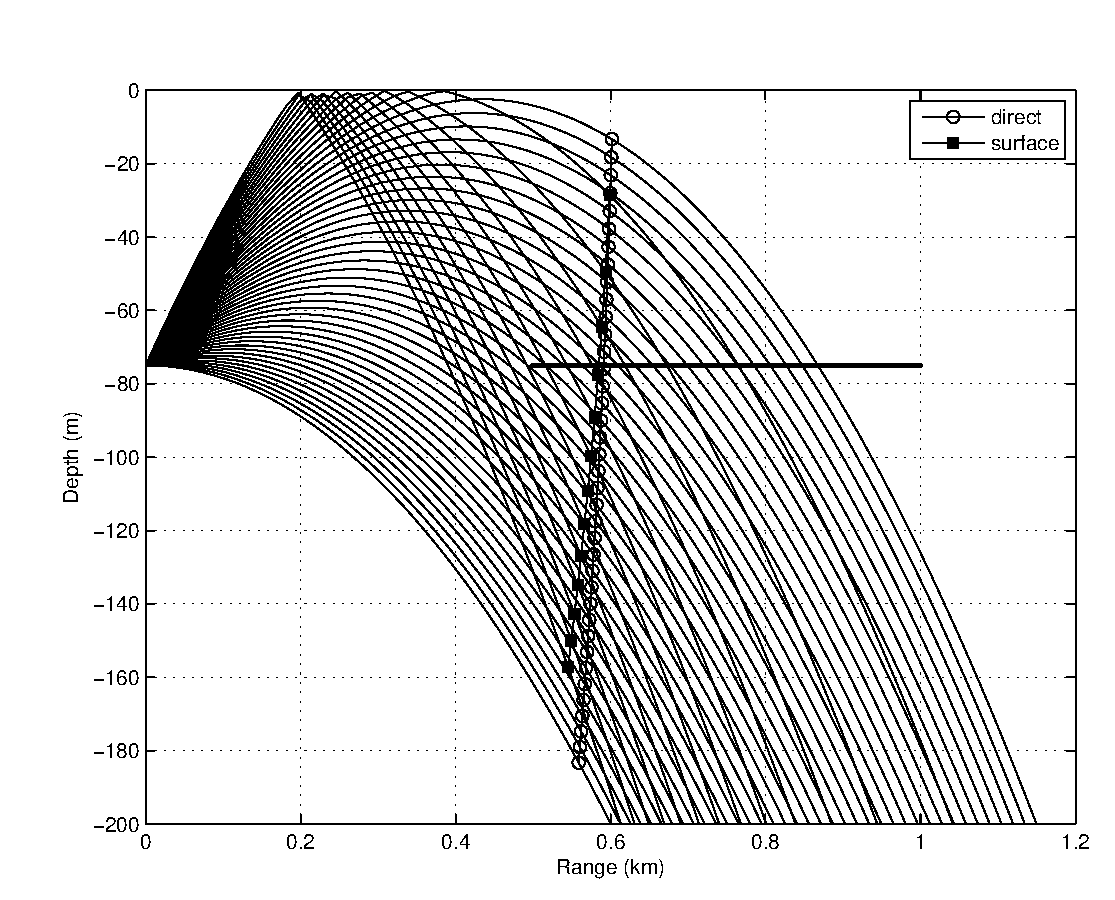
\includegraphics[width=4in]{pedersen_shallow_raytrace.eps}} 
	\vspace*{8pt}
	\caption{Ray trace for shallow source. 
	\label{fig:pedersen_shallow_raytrace}}
\end{figure}

Figures~\ref{fig:pedersen_shallow_compare1} and
\ref{fig:pedersen_shallow_compare2} compare the individual WaveQ3D and GRAB
eigenrays for the direct and surface reflected paths. Analytic solutions
for the travel time and rays angles were also computed using Eqn.
(\ref{eq:snells_sphr}) through (\ref{eq:snells_sphr_time_integ}). To highlight
differences in travel time, a bulk time has been removed using the slope of
the analytic solution for the direct path.  
\begin{figure}[th]
	\centerline{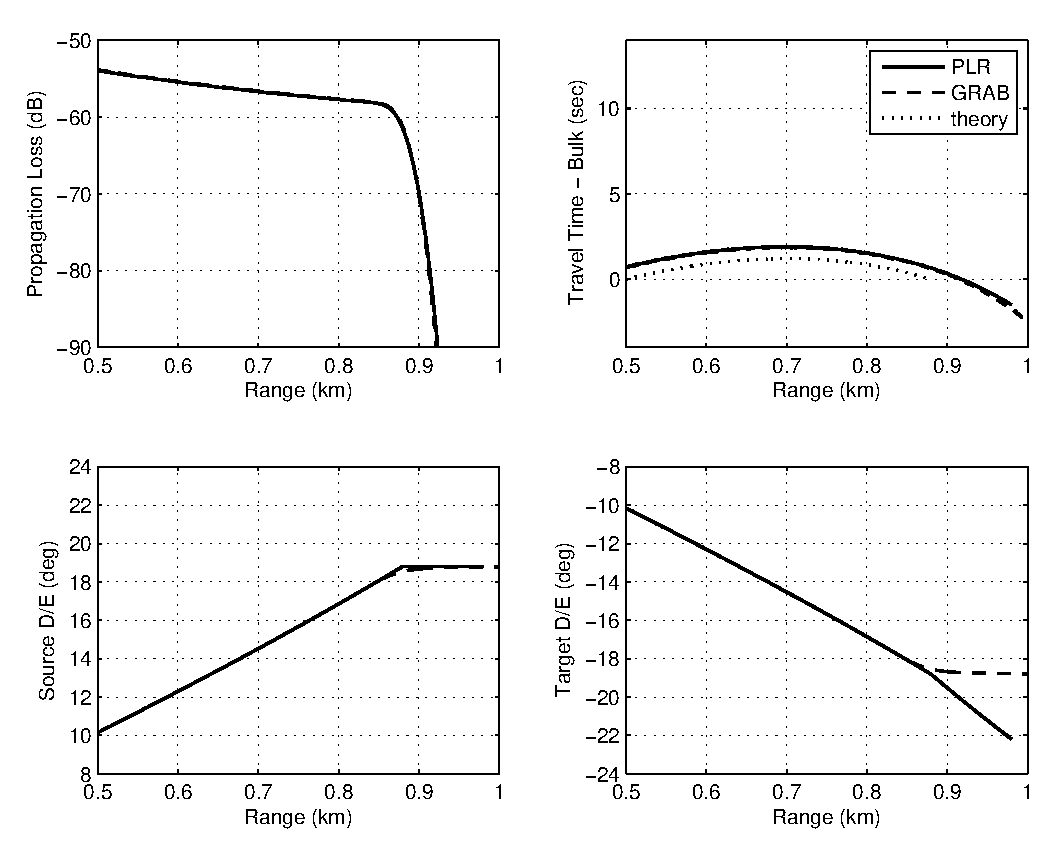
\includegraphics[width=4in]{pedersen_shallow_compare1.eps}} 
	\vspace*{8pt}
	\caption{Direct path eigenrays for shallow source. 
	\label{fig:pedersen_shallow_compare1}}
\end{figure}
\begin{figure}[th]
	\centerline{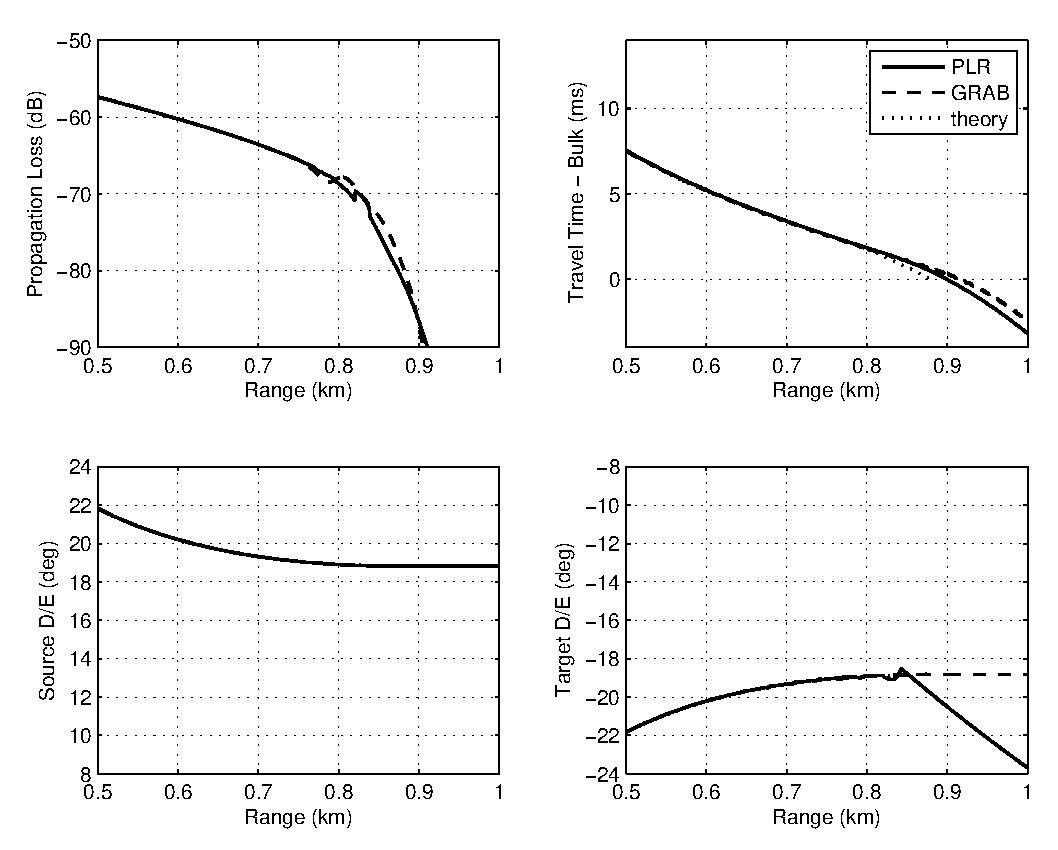
\includegraphics[width=4in]{pedersen_shallow_compare2.eps}} 
	\vspace*{8pt}
	\caption{Surface reflected eigenrays for shallow source. 
	\label{fig:pedersen_shallow_compare2}}
\end{figure}

The GRAB model was configured using ray fan with launch angles from
0\textsuperscript{0} to 25\textsuperscript{o} in 0.1\textsuperscript{o}
increments. However, it is important to note that, using the sound speed at
the source, GRAB automatically enhances the fan around the critical with 11
additional beams with spacings of 0\textsuperscript{o},
\(\pm\)0.03125\textsuperscript{o}, \(\pm\)0.0625\textsuperscript{o},
\(\pm\)0.125\textsuperscript{o}, \(\pm\)0.25\textsuperscript{o}, and
\(\pm\)0.5\textsuperscript{o}. If these small rays spacings were not used
near the critical ray, it would lead to un-realistically large gaps between
the outer edge of each ray family and the critical ray. This is especially
true for the surface reflected path in this geometry.

To achieve a similar effect, WaveQ3D was configured with
0.025\textsuperscript{o} spaced depression/elevation angles from
0\textsuperscript{o} to +25\textsuperscript{o} and 1\textsuperscript{o} spaced
azimuth angles from -4\textsuperscript{o} to +4\textsuperscript{o}. Because
this geometry evolves so quickly in time, the WaveQ3D results were created
using a 10~ms time step instead of the 100~ms value used in other tests. 

\begin{table}[th]
	\tbl{Individual eigenrays for shallow source. 
	\label{tab:pedersen_shallow_compare1}}
	{\begin{tabular}{@{}lcccccc@{}} \toprule
		Scenario & bias & deviation & r\textsuperscript{2} 
			& time & source DE & target DE \\ \colrule
		GRAB Direct & - & - & - 
			& 0.74 ms & 0.25\textsuperscript{o} & 0.25\textsuperscript{o} \\
		GRAB Surface & - & - & - 
			& 0.66 ms & 0.02\textsuperscript{o} & 0.02\textsuperscript{o} \\
		WaveQ3D Direct & +0.03 dB & \(\pm\)0.46 dB & 99.9\% 
			& 0.71 ms & 0.00\textsuperscript{o} & 0.00\textsuperscript{o} \\
		WaveQ3D Surface & 0.00 dB & \(\pm\)1.40 dB & 99.1\% 
			& 0.47 ms & 0.02\textsuperscript{o} & 0.99\textsuperscript{o} \\
			\botrule
	\end{tabular}}
\end{table}
Quantitative results for the shallow source's individual eigenrays are
summarized in Table~\ref{tab:pedersen_shallow_compare1}. In this table, the
maximum difference in travel time, source depression/elevation angle, and
target depression/elevation angle are computed relative to the analytic
solution. Those time and angle comparisons are limited to non-evanescent
regions, where the the analytic solutions had real values. Because our
analytic solution did not support propagation loss for individual
eigenrays, WaveQ3D values were compared to GRAB in this table.

From these results, we conclude that GRAB and WaveQ3D have similar eigenray
accuracy when compared to analytic solutions. In this case, the major
difference appears to be differences in the way that GRAB and WaveQ3D
handle depression/elevation angles near the shadow zone. GRAB's angles are a
weighted sum of contribution from neighboring Gaussian beams. This gives
GRAB a smooth roll-off from angles inside the ray fan to a constant value
on the outside. GRAB's constant value is taken from the closest ray in
horizontal range. In contrast, the WaveQ3D angles are computed from the
geometry of eigenray offsets. Outside of the ray fan, WaveQ3D uses angles from
the ray that is closest in slant range. Because the rays in this geometry
are rapidly changing direction near the shadow zone, the difference between
slant and horizontal range results in WaveQ3D target depression/elevation
angles that are up to 4\textsuperscript{o} different than the GRAB result.
But because the analytic solution is not valid in this region, that
difference is not reflected in Table~\ref{tab:pedersen_shallow_compare1}.

\begin{figure}[th]
	\centerline{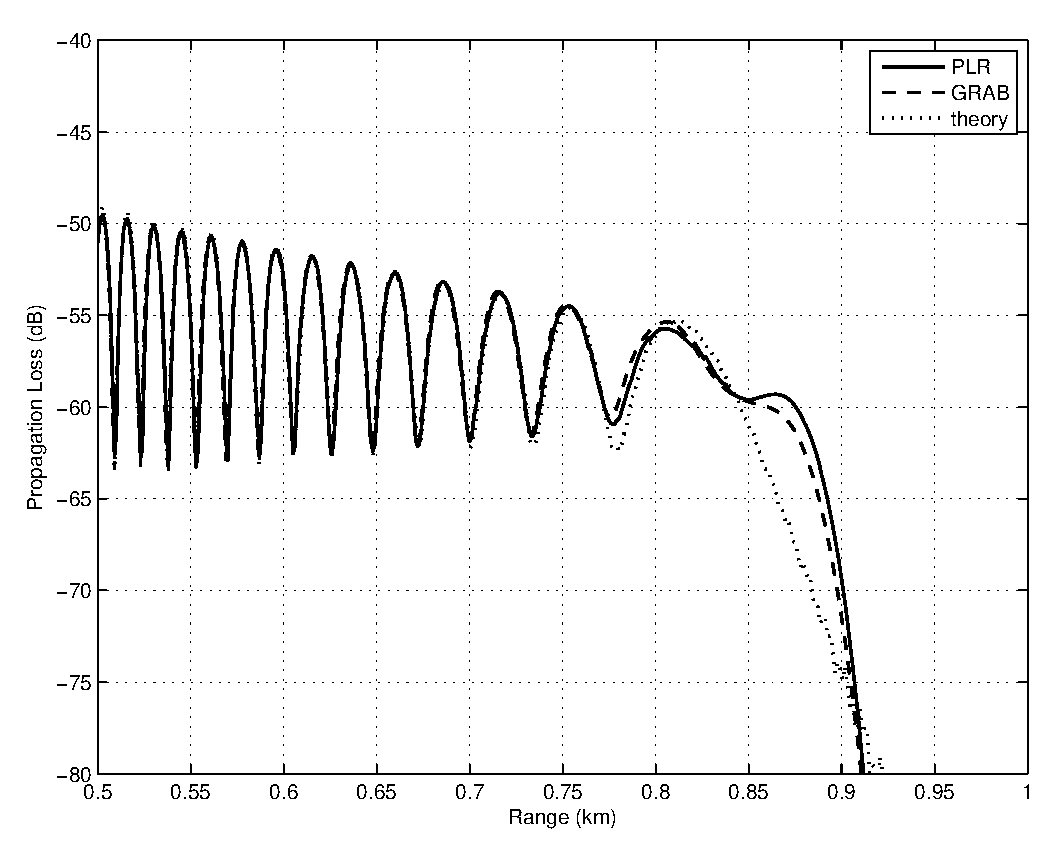
\includegraphics[width=3in]{pedersen_shallow_compare3.eps}} 
	\vspace*{8pt}
	\caption{Propagation loss for shallow source. 
	\label{fig:pedersen_shallow_compare3}}
\end{figure}
Differences in total propagation loss for the shallow source geometry are
illustrated in Fig.~\ref{fig:pedersen_shallow_compare3} and summarized in
Table~\ref{tab:pedersen_shallow_compare3}. The analytic solution for this
test were computing using the Fast Field Program (FFP) wavenumber
integration technique.\cite{DiNapoli1980,Brekhovskikh1980} Note that, in
all regions, this implementation of FFP was consistent with an ideal wave
equation solution, except for the presence of some implementation jitter in
the ranges above 880~m. In the region between 500-750 m, all three models
produced almost identical results. As target passed into the shadow zone
region, WaveQ3D and GRAB produced values that were similar to each other,
but slightly higher than FFP. But we also noted that, if a coarser set of
depression elevation launch angles was used for WaveQ3D, the surface
reflected path would have disappeared prematurely, which would have
manifested as shadow zone oscillations in the total propagation loss. Taken
as a whole, we feel confident that Wave3D propagation loss errors are
similar to those of GRAB for this scenario.
\begin{table}[th]
	\tbl{Total propagation loss for shallow source. 
	\label{tab:pedersen_shallow_compare3}}
	{\begin{tabular}{@{}lcccccc@{}} \toprule
		Scenario & bias & deviation & r\textsuperscript{2} \\ \colrule
		GRAB & +0.71 dB & \(\pm\)1.78 dB & 92.5\% \\
		WaveQ3D & +0.80 dB & \(\pm\)2.21 dB & 88.7\% \\
		GRAB \(\leq\) 0.75 km & +0.09 dB & \(\pm\)0.58 dB & 97.7\% \\
		WaveQ3D \(\leq\) 0.75 km & -0.03 dB & \(\pm\)0.47 dB & 98.4\% \\
	\end{tabular}}
\end{table}

\subsection*{Deep source geometry}

Figure~\ref{fig:pedersen_deep_raytrace} is a ray trace for the deep source
geometry. 
\begin{figure}[th]
	\centerline{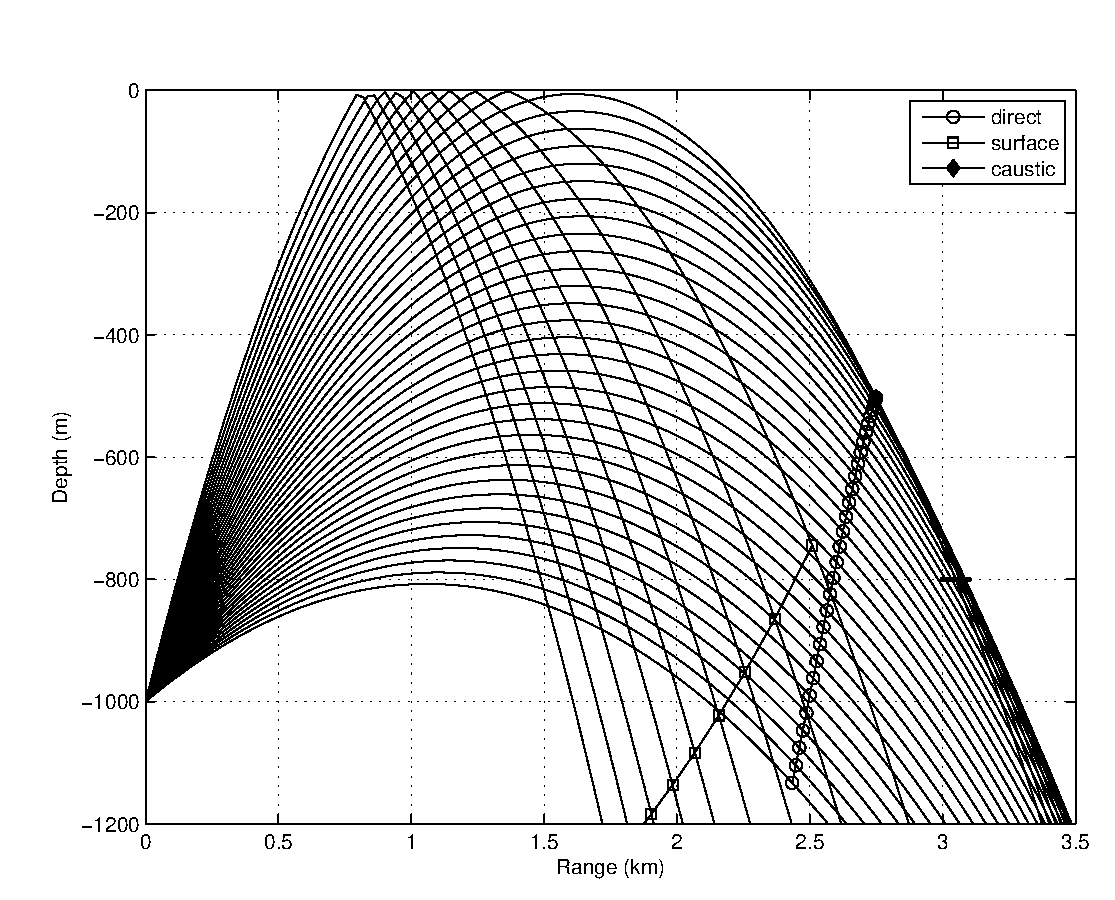
\includegraphics[width=3in]{pedersen_deep_raytrace.eps}} 
	\vspace*{8pt}
	\caption{Ray trace for shallow source. 
	\label{fig:pedersen_deep_raytrace}}
\end{figure}
This plot illustrates a ray fan with launch angles from
20\textsuperscript{0} to 60\textsuperscript{o} in 1\textsuperscript{o}
increments. The target locations are illustrated by the horizontal black
line. There are three potential eigenrays for each target. Rays launched
above the critical angle (51.21\textsuperscript{0}) hit the surface before
ensonifying the target. However, because all of the surface reflected paths
are far from the targets, their contribution to the overall solution is
weak. Starting at around 2.5 seconds of travel time, the outer edge of the
wavefront folds back on itself and splits the remaining contributions into
strong direct path and caustic ray families. The direct path, surface
reflected, and caustic components of the wavefront at 2.5 sec are
illustrated with circle, square, and diamond symbols on
Fig.~\ref{fig:pedersen_deep_raytrace}.

\begin{figure}[th]
	\centerline{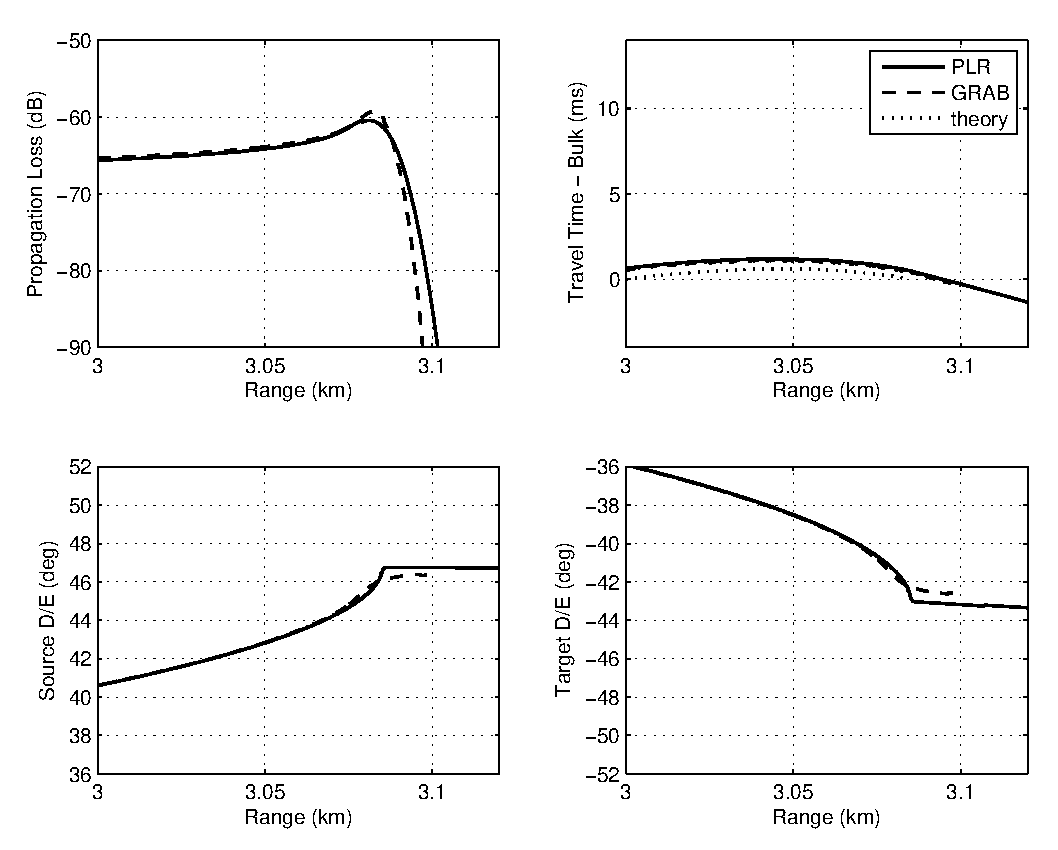
\includegraphics[width=4in]{pedersen_deep_compare1.eps}} 
	\vspace*{8pt}
	\caption{Caustic eigenrays for deep source. 
	\label{fig:pedersen_deep_compare1}}
\end{figure}
\begin{figure}[th]
	\centerline{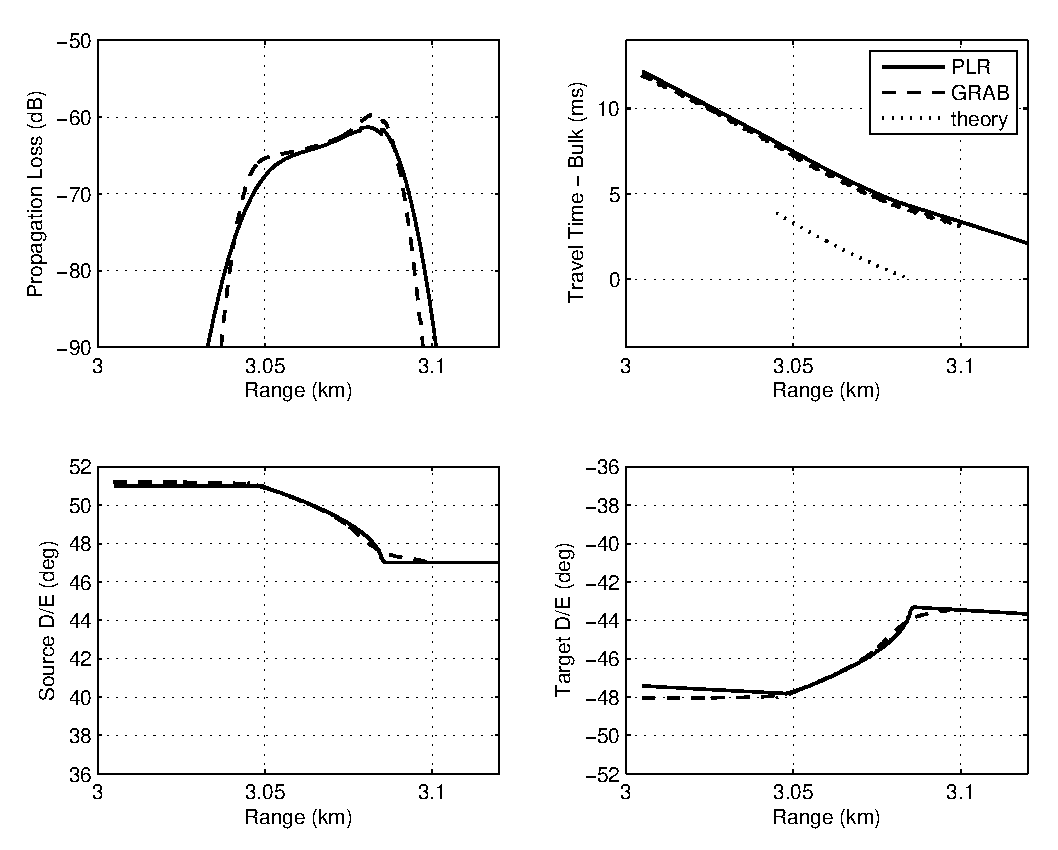
\includegraphics[width=4in]{pedersen_deep_compare2.eps}} 
	\vspace*{8pt}
	\caption{Direct path eigenrays for deep source. 
	\label{fig:pedersen_deep_compare2}}
\end{figure}

Figures~\ref{fig:pedersen_deep_compare1} and
\ref{fig:pedersen_deep_compare2} compare the individual WaveQ3D and GRAB
eigenrays for the deep source's direct and caustic paths. As before, a bulk
time has been removed using the slope of the analytic solution for the
direct path. In these results, the GRAB model was configured using ray fan
with launch angles from 20\textsuperscript{0} to 60\textsuperscript{o} in
0.1\textsuperscript{o} increments and rays near the caustic were
automatically augmented. WaveQ3D used a ray spacing of
0.25\textsuperscript{o} spacing to achieve a similar result.

The big difference between the models appears to be the fact that the
WaveQ3D transmission loss has a more gradual roll-off into the shadow zones
than GRAB. Quantitative comparisons for the deep source's individual
eigenrays are summarized in Table~\ref{tab:pedersen_deep_compare1}. The
statistics for the WaveQ3D angles for the caustic path are skewed by the
fact that differences in launch angle resolutions causes inner edge of the
WaveQ3D result to prematurely transition to it shadow zone result. In other
regions, the agreement is much closer. It is also important to note that
the depression/elevation angle deviations seen in the WaveQ3D results for
the shallow source are less evident in the deep source case.
\begin{table}[th]
	\tbl{Individual eigenrays for deep source. 
	\label{tab:pedersen_deep_compare1}}
	{\begin{tabular}{@{}lcccccc@{}} \toprule
		Scenario & bias & deviation & r\textsuperscript{2} 
			& time & source DE & target DE \\ \colrule
		GRAB Direct & - & - & - 
			& 0.65 ms & 0.47\textsuperscript{o} & 0.54\textsuperscript{o} \\
		GRAB Caustic & - & - & - 
			& 3.77 ms & 0.87\textsuperscript{o} & 0.98\textsuperscript{o} \\
		WaveQ3D Direct & +0.06 dB & \(\pm\)3.17 dB & 97.0\% 
			& 0.64 ms & 0.21\textsuperscript{o} & 0.24\textsuperscript{o} \\
		WaveQ3D Caustic & +1.15 dB & \(\pm\)4.07 dB & 94.4\% 
			& 3.97 ms & 1.24\textsuperscript{o} & 1.40\textsuperscript{o} \\
			\botrule
	\end{tabular}}
\end{table}

Differences in total propagation loss for the deep source geometry are
illustrated in Fig.~\ref{fig:pedersen_deep_compare3} and summarized in
Table~\ref{tab:pedersen_deep_compare3}. In the region from 3000 to 3040
meters, the FFP has stronger oscillations than either the WaveQ3D or GRAB
models. This can be attributed to surface reflected contribution that is
stronger in the FFP result than in either of the Gaussian beam models. At
all other ranges, the WaveQ3D and GRAB results were both a very close fit
to FFP's total propagation loss.
\begin{figure}[th]
	\centerline{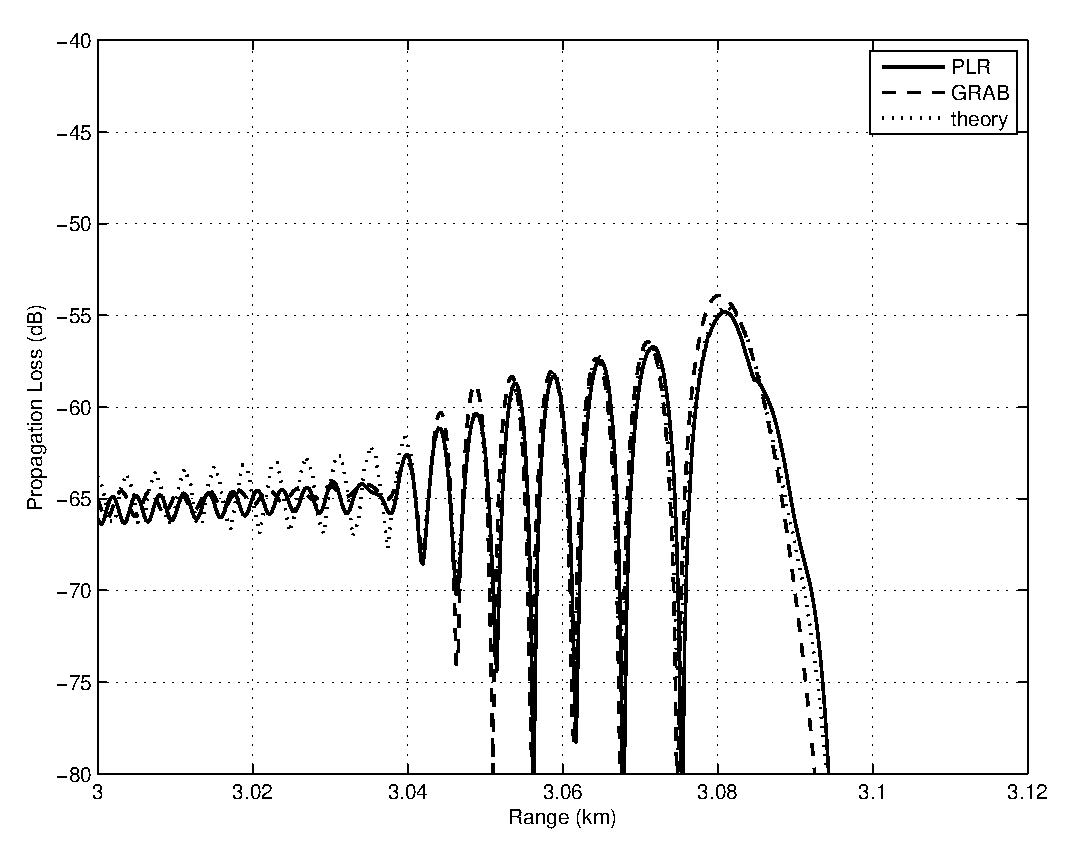
\includegraphics[width=3in]{pedersen_deep_compare3.eps}} 
	\vspace*{8pt}
	\caption{Propagation loss for deep source. 
	\label{fig:pedersen_deep_compare3}}
\end{figure}

\begin{table}[th]
	\tbl{Total propagation loss for deep source. 
	\label{tab:pedersen_deep_compare3}}
	{\begin{tabular}{@{}lcccccc@{}} \toprule
		Scenario & bias & deviation & r\textsuperscript{2} \\ \colrule
		GRAB & -0.95 dB & \(\pm\)3.05 dB & 95.4\% \\
		WaveQ3D & -0.22 dB & \(\pm\)1.94 dB & 92.8\% \\
		GRAB \(\geq\) 3.04 km & -1.45 dB & \(\pm\)3.70 dB & 97.0\% \\
		WaveQ3D \(\geq\) 3.04 km & -0.03 dB & \(\pm\)2.20 dB & 94.4\% \\
	\end{tabular}}
\end{table}
A WaveQ3D anomaly was discovered during the deep source geometry testing.
Errors in the total propagation loss within the shadow zone were frequently
seen when the launch angles finer than 0.01 degrees were used. What we
discovered was that at this spacing, the contribution in the shadow zone
was the result of a summation of over 100 Gaussian beams for both the
direct and caustic paths. Small errors in the calculation of cell width and
cell distance to the target appear to accumulate when the total loss is the
result of many weak contributions. For the individual eigenrays, this
anomaly results in a slight broadening of the transmission loss decay
tails. But, since the shape of the outer edge of the total propagation loss
depends on destructive interference between the paths, these errors often
resulted in imperfect cancellation, on the order of -70 dB, in the region
between 3090 and 3105 meters. Although these problems may have been
aggravated by the extreme environment, developers should use extra caution
when using WaveQ3D with super-fine ray spacings.

\section{Summary}

This paper represents an important milestone the development of the WaveQ3D
model. A suite of tests were developed to quantitatively compare the ray
tracing, reflection, eigenray finding, and propagation loss elements of the
model to analytic solutions. Hopefully, this approach will help other
researchers evaluate the capability and limitations of the WaveQ3D model
and provide a firm foundation to move forward with further testing.

This testing also led to the development of a few general guidelines for the
use of the WaveQ3D model.
\begin{itemlist}
\item Using a time step size as coarse as 100~ms seems to produce accurate
results for most applications. However, this step size should be decreased
to 10~ms for applications that need high accuracy at ranges less than 2~km.
This is particularly true for applications that are interested in effects
near the ocean surface, or directly below the source.
\item The selection of launch angles can have a significant effect on
propagation loss results. Like all models that as based on ray theory, WaveQ3D
can miss features in the environment because of spatial under-sampling.
Tangent spaced depression/elevation angles appear to improve WaveQ3D model
performance for scenarios dominated by horizontal paths. Uniform spacing is
suggested for applications that need high accuracy at ranges less than
2~km.
\item The WaveQ3D model is designed to be computationally efficient when
computing transmission loss for up to 100 targets, at multiple frequencies,
in a fully 3-D environment. But because the WaveQ3D eigenray detection
process is less efficient than an equivalent calculation in Cartesian
coordinates, WaveQ3D can actually be much slower than other models when
thousands of range/depth combinations are required. Applying the WaveQ3D
model in 2-D environments is also not very efficient.
\end{itemlist}

\section*{Acknowledgments}

This paper was developed as part of Sean Reilly's PhD studies at the Ocean
Engineering Department of the University of Rhode Island, under the
direction of Dr. Gopu Potty and Dr. James Miller. This verification testing
effort was funded by the High Fidelity Active Sonar Training (HiFAST)
Project at the U.S. Office of Naval Research.

\appendix

\section{Ray path derivation for concave ocean surface}

The analytic solution for the direct-path eigenrays was derived from the
laws of sines and cosines.
\begin{equation}
	a^2 = r_1^2 + r_2^2 - 2 r_1 r_2 cos( \Delta \theta ) \:,
	\label{eq:eigenray_lloyds_a}
\end{equation}
\begin{equation}
	t_d = a / c_0 \:,
	\label{eq:eigenray_lloyds_tdirect}
\end{equation}
\begin{equation}
	\mu_{d,source} = - arcsin \left( \frac{a^2+r_1^2-r_2^2}{2 a r_1} \right) \:,
	\label{eq:eigenray_lloyds_mus}
\end{equation}
\begin{equation}
	\mu_{d,target} = arcsin \left( \frac{a^2+r_2^2-r_1^2}{2 a r_2} \right) \:,
	\label{eq:eigenray_lloyds_mut}
\end{equation}
where 
\( t_d \) is the direct-path travel time from source to target;
\( \mu_{d,source} \) is the direct-path depression/elevation angle at source; and
\( \mu_{d,target} \) is the direct-path depression/elevation angle at target.

The analytic solution for the surface reflected solution also starts with
the law of cosines.
\begin{equation}
	\cos{\beta} = \frac{R^2 + b_1^2 - r_1^2}{2 R b_1} 
		= \frac{R^2 + b_2^2 - r_2^2}{2 R b_2} \:.
	\label{eq:surf_1}
\end{equation}
This can be reduced to a simpler form using
\begin{equation}
	R^2 + b_n^2 - r_n^2 
		= R^2 + (R^2 + r_n^2 - 2 R r_n cos(\Delta \theta_n) ) - r_1^2 
		=  2 R ( R - r_n cos(\Delta \theta_n) )
	\label{eq:surf_2}
\end{equation}
to yield
\begin{equation}
	\cos{\beta} = \frac{R - r_1 cos(\Delta \theta_1)}{b_1} 
		= \frac{R - r_2 cos(\Delta \theta_2)}{b_2} \:.
	\label{eq:surf_3}
\end{equation}
When this is combined with the law of sines
\begin{equation}
	\sin{\beta} = \frac{r_1 sin(\Delta \theta_1)}{b_1} 
		= \frac{r_2 sin(\Delta \theta_2)}{b_2}\:,
	\label{eq:surf_4}
\end{equation}
it yields an analytic relationship between the source/target depths and the
angles (\(\Delta \theta_1, \Delta \theta_2\)) at which reflections occur
\begin{equation}
	\frac{\cos{\beta}}{\sin{\beta}} 
		= \frac{ R/r_1 - cos(\Delta \theta_1)}{sin(\Delta \theta_1)} 
		= \frac{ R/r_2 - cos(\Delta \theta_2)}{sin(\Delta \theta_2)} \:,
	\label{eq:surf_5}
\end{equation}
\begin{equation}
	\frac{R}{r_1} sin(\Delta \theta_2) - sin(\Delta \theta_2) cos(\Delta \theta_1)
	 = \frac{R}{r_2} sin(\Delta \theta_1) - cos(\Delta \theta_2) sin(\Delta \theta_1) \:,
	\label{eq:surf_6}
\end{equation}
\begin{equation}
	r_1 sin( \Delta \theta_1 ) - r_2 sin( \Delta \theta_2 ) 
		+ \frac{r_1 r_2}{R} sin( \Delta \theta_2 - \Delta \theta_1 ) = 0  \:.
	\label{eq:surf_7}
\end{equation}

The analytic solutions for the surface reflected path requires finding values of \( \Delta \theta_1 \) which solve the transcendental equation
\begin{equation}
	r_1 sin( \Delta \theta_1 ) - r_2 sin( \Delta \theta - \Delta \theta_1 ) 
		+ \frac{r_1 r_2}{R} sin( \Delta \theta - 2 \Delta \theta_1 ) = 0 \:.
	\label{eq:surf_8}
\end{equation}

\section{Tangent spaced depression/elevation angles}

\begin{figure}[th]
	\centerline{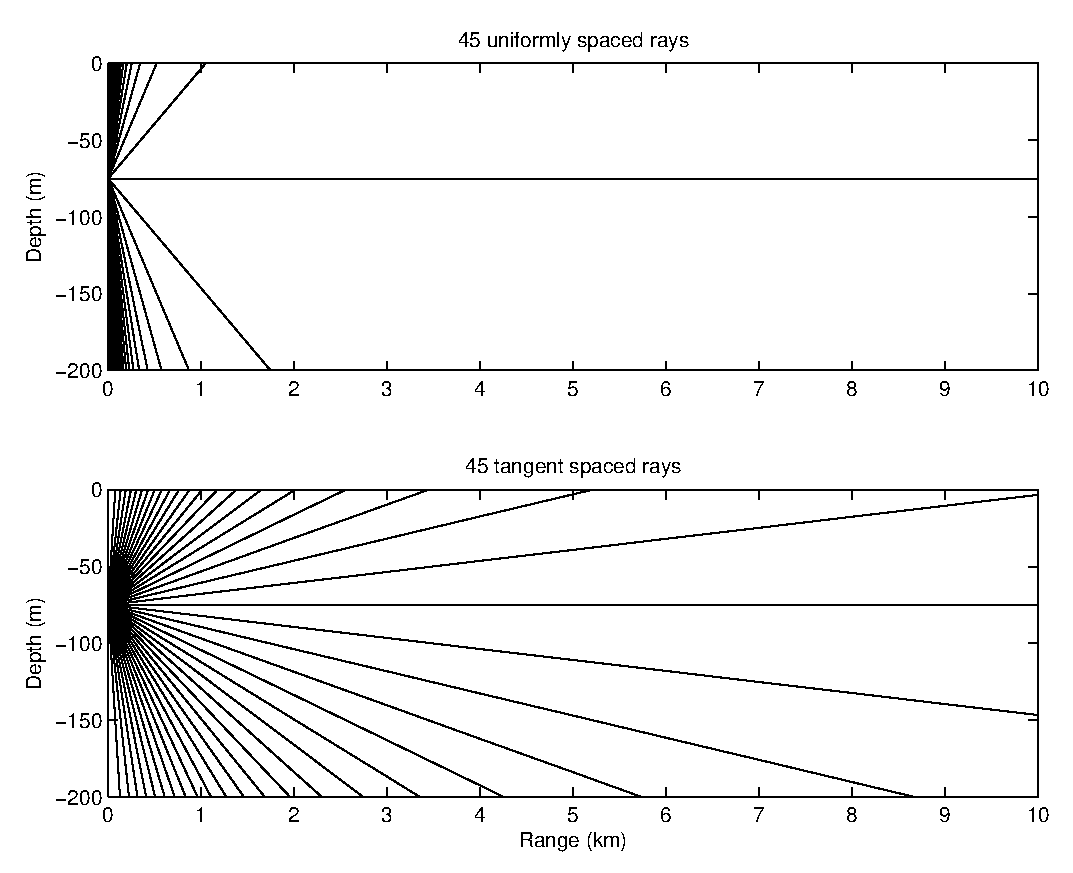
\includegraphics[width=3in]{plot_seq_rayfan.eps}} 
	\vspace*{8pt}
	\caption{Tangent spaced beams.  
	\label{fig:plot_seq_rayfan}}
\end{figure}
Because sonar detection ranges are often much longer than the depths of
interest, there is frequently a need to emphasis propagation paths near the
horizontal. The GRAB model\cite{GRAB2008} manages this requirement by
automatically adding rays in the depression/elevation directions needed to
support caustics, surface ducts, and SOFAR channels. The WaveQ3D model
currently does not support any such automatic ray adjustment; but it does
support any ray spacing that is monotonically increasing.

Tangent spaced depression/elevation angles will be used frequently in the
eigenray and propagation loss testing for WaveQ3D. As shown in the top panel of
Fig.~\ref{fig:plot_seq_rayfan}, uniformly spaced rays in an isovelocity
environment severely under-sample the direct path contributions at ranges
beyond a few kilometers. When the ray paths are initialized such that the
tangents of the launch angles are uniformly spaced (bottom panel), the long
range contributions are better supported. Of course, this improvement comes
at the expense of short range contributions. But, that trade-off often
matches the requirements of sonar simulations.

To generate a set of N tangent spaced beams \(\mu[n]\), over the interval [\(\mu_1,\mu_N\)], with the densest spacing at \(\mu_c\), WaveQ3D uses the following algorithm
\begin{equation}
	a_1 = arctan \left( \frac{\mu_1-\mu_c}{\sigma} \right)
\end{equation}
\begin{equation}
	a_N = arctan \left( \frac{\mu_N-\mu_c}{\sigma} \right)
\end{equation}
\begin{equation}
	x[n] = a_1 +\frac{a_N-a_1}{N-1} n \quad \text{for n = 0, 1, 2, ..., N-1}
\end{equation}
\begin{equation}
	\mu[n] = \mu_c + \sigma \: tan(x[n])
\end{equation}
where
\(\sigma\) is an arbitrary scaling factor.  WaveQ3D testing frequently uses 181 tangent spaced depression/elevation rays, from -90\textsuperscript{o} to +90\textsuperscript{o}, with 
\(\mu_c=0\)\textsuperscript{o} and \(\sigma=6\).  This combination of factors yields a ray fan with maximum resolution of about 0.1\textsuperscript{o} and 85\% of its rays in the \(\pm\)20\textsuperscript{o} range.

\section{Propagation loss error statistics}

We would like to define quantitative differences between modeled and analytic propagation losses in a way that illuminates the suitability of the model for real-time, sonar simulation/stimulation systems.  To that end, we define the following statistical measures
\begin{equation}
	b[PL] = \frac{1}{N} \sum^N_{n=1} ( PL_{model}[n] - PL_{theory}[n] ) \:,
	\label{eq:bias_calc}
\end{equation}
\begin{equation}
	\psi^2[PL] = \frac{1}{N} \sum^N_{n=1} 
		( PL_{model}[n] - PL_{theory}[n] )^2 \:,
\end{equation}
\begin{equation}
	s[PL] = \sqrt{ \psi^2[PL] - b^2[PL] } \:,
	\label{eq:dev_calc}
\end{equation}
\begin{equation}
	x[n] = PL_{theory}[n] - \frac{1}{N} \sum^N_{n'=1} ( PL_{theory}[n'] \:,
\end{equation}
\begin{equation}
	y[n] = PL_{model}[n] - \frac{1}{N} \sum^N_{n'=1} ( PL_{model}[n'] \:,
\end{equation}
\begin{equation}
	r^2[PL] =  \frac{ \left( \sum\limits^N_{n=1} x[n] y[n] \right)^2 }
	                   { \sum\limits^N_{n=1} x^2[n] \sum\limits^N_{n=1} y^2[n] } 
	                   \times 100\% \:,
	\label{eq:r2_calc}
\end{equation}
where
\(PL_{model}[n]\) and \(PL_{theory}[n]\) are the samples in the model and theory in dB units;
$b[PL]$ is the estimated bias between the model and the theory;
$s[PL]$ is the estimated deviation between the model and the theory; and
\(r^2[PL]\) is the coefficient of determination between the model and the theory.

The active sonar equation can be expressed in the form
\begin{equation}
	SE = FOM - 2 PL \:,
\end{equation}
\begin{equation}
	FOM = SL + TS - NL + DI - DT \:,
\end{equation}
where
SE is the signal excess;
PL is the propagation loss;
FOM is the active figure of merit;
SL is the source level;
TS is the target strength;
NL is the noise level;
DI is the directivity index; and
DT is the detection threshold.\cite{Urick1983}
If we assume that errors in the figure of merit are handled separately,
then \(2 b[PL]\) and \(s^2[PL]\) are estimates of signal excess bias and
variance. The coefficient of determination, \(r^2[PL]\), estimates how well
the modeled signal excess' shape is correlated to an ideal solution.

\begin{thebibliography}{0}

\bibitem{Reilly2012} S. M. Reilly, G. Potty, Sonar Propagation Modeling using Hybrid
Gaussian Beams in Spherical/Time Coordinates, Department of Ocean Engineering, University of Rhode Island, January 2012.

\bibitem{Veldhuizen1995} T. Veldhuizen, "Expression Templates," C++ Report,
Vol. 7 No. 5 June 1995, pp. 26-31

\bibitem{Chrissis2007} M. B. Chrissis, M. Konrad, S. Shurm, {\bf CMMI
Guidelines for Process Integration and Product Development}, Second
Edition, (Addison-Wesley, New York, 2007).

\bibitem{Yakowitz1986} Yakowitz and Szidarovszky, {\bf An Introduction to
Numerical Computation} (Macmillan Publishing, New York, 1986) pp. 306-311.

\bibitem{Pekeris1946} C. L. Pekeris, Accuracy of the Earth-Flattening
Approximation in the Theory of Microwave Propagation, {\it Phys. Rev.} {\bf
70} (1943).

\bibitem{Munk1974} W. H. Munk, Sound channel in an exponentially stratified
ocean, with application to SOFAR, {\it J.~Acoust. Soc. Amer.} {\bf 55}
(1974) pp. 220-226.

\bibitem{Jensen1994} F. B. Jensen, W. A. Kuperman, M. B. Porter, and H.
Schmidt, {\bf Computational Ocean Acoustics}, {\it American Institute of
Physics Press, New York} (1994).

\bibitem{Porter1997} M.B.Porter, The KRAKEN Normal Mode Program (DRAFT),
A Deep Water Problem: the Munk Profile (1997)
http://oalib.hlsresearch.com/Modes/AcousticsToolbox/manual\_html/node8.html.

\bibitem{Cerveny2001} V. Cerveny, {\bf Seismic Ray Theory}, (Cambridge
University Press, New York, 2001), pp.174-178.

\bibitem{Shampine2010} L.F. Shampine, Vectorized Adaptive Quadrature in
MATLAB, {\it J.~Comput. Appl. Math.} {\bf 70} (2008).

\bibitem{Williams2011} E. Williams, Aviation Formulary V1.46,
http://williams.best.vwh.net/avform.htm, 2011

\bibitem{Pedersen1972} M. A. Pedersen, D. F. Gordon, Normal-Mode and Ray
Theory Applied to Underwater Acoustic conditions of Extreme Downward
Refraction, {\it J.~Acoust. Soc. Amer.} {\bf 51} (1972) 323.

\bibitem{Porter1987} M. B. Porter, H. P. Bucker, Gaussian beam tracing for
computing ocean acoustic fields, {\it J.~Acoust. Soc. Amer.} {\bf 93}
(1987) 1349.

\bibitem{Weinberg1996} H. Weinberg, R. E. Keenan, Gaussian ray bundles for
modeling high-frequency propagation loss under shallow-water conditions,
{\it J.~Acoust. Soc. Amer.} {\bf 100} (1996) 1421.

\bibitem{ETOPO1} ETOPO1v2 Global Gridded 2-minute Database, National
Geophysical Data Center, National Oceanic and Atmospheric Administration,
U.S. Dept. of Commerce, http://www.ngdc.noaa.gov/mgg/global/ETOPO1.html.

\bibitem{Sturm2008} F. Sturm, S. Ivansson, Y. M. Jiang, N. R. Chapman,
Numerical investigation of out-of-plane sound propagation in a shallow
water experiment, {\it J.~Acoust. Soc. Amer.} {\bf 124} (2008) pp. 341-346.

\bibitem{GRAB2008} Software Requirements Specification/Software Design
Description and Software Test Description for the Oceanographic and
Atmospheric Master Library Navy Standard Comprehensive Acoustic System
Simulation Model Version 4.2A, {\it Naval Meteorology and Oceanography
Command Report OAML-SRS-SDD-STD-83D} (2008).

\bibitem{DiNapoli1980} F. R. DiNapoli, R. L. Deavenport, Theoretical and
numerical Green's function field solution in a plane multilayered medium,
{\it J. Acoust. Soc. Amer.} {\bf 67} (1980).

\bibitem{Brekhovskikh1980} L. M. Brekhovskikh, Waves in Layered Media
(Academic Press Inc., New York, 1980), 2nd Edition, Section 54.

\bibitem{Urick1983} R. J. Urick, {\bf Principles of underwater sound, 3rd
edittion}, {\it McGraw-Hill, New York} (1983).

\end{thebibliography}
\end{document}

